% Chapter 4
\chapter{Methodology} % Main chapter title
\label{Chapter4} % For referencing the chapter elsewhere, use \ref{Chapter2} 
\minitoc
%----------------------------------------------------------------------------------------

%% Define some commands to keep the formatting separated from the content 
%\newcommand{\keyword}[1]{\textbf{#1}}
%\newcommand{\tabhead}[1]{\textbf{#1}}
%\newcommand{\code}[1]{\texttt{#1}}
%\newcommand{\file}[1]{\texttt{\bfseries#1}}
%\newcommand{\option}[1]{\texttt{\itshape#1}}
%----------------------------------------------------------------------------------------

This chapter is devoted to the description of the software framework developed to solve the problem proposed in \ref{Chapter1}. This work proposes a solution based on Big-Data database, python scripts and exploratory visualizations that allows a solution using Gaussian Hidden Markov Model and hierarchical agglomerative clustering. Finally, at the end of this chapter, we evaluate each of the proposed models to observe the different results that we achieve with each one.

\section{Software Framework}

\paragraph{Identifying the problem scenario}
We consider that the unsupervised fault detection by using machine learning in a multivariate building dataset is a problem that falls in different domains. Regarding the variety of the time series, we consider this problem as a Big-Data problem, since IoT \footnote{IoT is including building and industrial control systems. There is still a question: 'Will we have a smart BAS in the future or is it just part of the IOT?'} is allowing to collect data from ubiquitous sensors, therefore criteria of volumen, variety and velocity are present \cite{george2014big,gubbi2013internet}. Regarding the discovery process of daily profiles, each daily profile is a sub-sequence of the whole trend, and finding the common patterns in the whole trend is analogous to the sub-sequence analysis of DNA sequences, for instance \cite{haussler1996generalized, ghahramani2001introduction, stamp2004revealing, ramage2007hidden, pfundstein2011hidden}. Finally, regarding data mining and visualization mechanisms, we consider that this problem requires effective techniques for knowledge discovery and expressive data visualization artifacts that fits the data \cite{witten2016data,aparicio2014, kohavi2001data}.   

\paragraph{Proposed solution}
We use MongoDB \footnote{For more information: \url{https://www.mongodb.com/what-is-mongodb}} database for having a smart manage of the dataset, the measures and calculations are stored as JSON-like documents allowing flexibility to save/retrieve the data as it was explained in section \ref{sec:dealing}. The architecture of the proposed solution is a traditional three-tier architecture powered by Python's scripts: a big-data database, an application web server and the front-end tier that is the browser's user. Figure \ref{fig:framework} shows the flow of information. The data processing step is done by a transversal script \footnote{script in: /Thesis\_project/lib/rs\_common\_framework\_v4.py} that provides the primitive methods for the all the different modules that are connected. The proposed solution allows the following data mining actions:

\begin{itemize}
\item[a] Raw Data Screening process: Filter values that do not belong to measuring process of the variable.
\item[b] Correlation analysis of variables: Construct a matrix of linear correlation of the variables of the multivariate dataset. \footnote{This process is explained inside of the interactional model, section \ref{sec:interactional_model}}
\item[c] Feature selection process: Calculate the gain of information of an arbitrary feature.
\item[d] Modeling process: The training process of the models, the best models are stored for latter uses. \footnote{ GaHMM models are saved as \textit{.pkl} files in folder: \textit{/Thesis\_project/HMM\_models/Final\_models}. The description of each model is in \textit{description\_model.txt.} }
\item[e] Visualization process: Two visualization mechanism are proposed. \textbf{1.} \textit{Jupyter notebook} \footnote{We use the python version. More available information in \url{http://jupyter.org/}.} is an open-source web application that allows to create and share documents that contain live code, equations, visualizations and explanatory text. \textbf{2} Flask web server \footnote{Web server is implemented using Flask for Python. \url{http://flask.pocoo.org/}} is an open-source web framework that is based on Werkzeug, Jinja 2. This micro-framework is compatible with other libraries like \textit{queue.js, jQuery.js, d3.js, bootstrap.js} that are used to generated personalized information visualizations. 

\end{itemize}

\begin{figure}[h!]
  \vspace{0.5em} %better style
  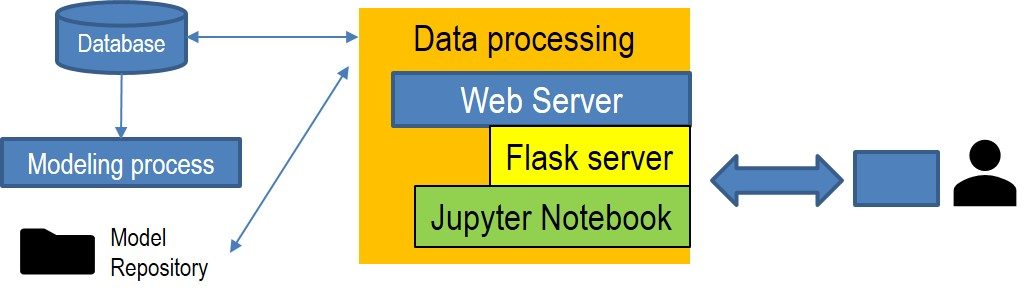
\includegraphics[scale=0.4]{Figures/framework.jpg}
  \caption{Software framework schema}
  \label{fig:framework}
\end{figure}

Figure \ref{fig:structure} shows the implemented collection of JSON documents that were created for each proposed module according to the last list of data mining actions, each of them are explained in details in the next sections.

\begin{figure}[h!]
  \vspace{0.5em} %better style
  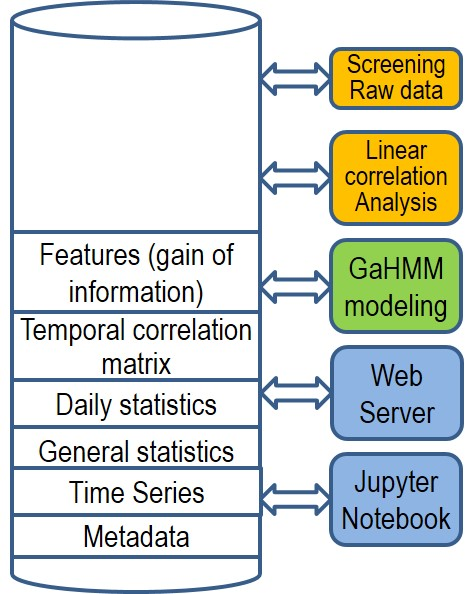
\includegraphics[scale=0.4]{Figures/database_structure.jpg}
  \caption{Implemented collections for saving time series and results}
  \label{fig:structure}
\end{figure} 
 
%We believe that the occupants behavior is a sequence of events during the day, and those sequences can be interpreted as states. For example, consider the following states: arrival at the office, breakfast (or small break), first working period, lunch, second working period, departure from the office. These states are a common sequence for people that work in an office building. We consider atypical days, those day where one or more of these states were skipped.  



\section{Raw Data Screening process}

The raw data screening process is an important step to do before performing any action over the time series dataset. Aspects like the definition of limits and the quality of the data are important issues to know before starting the knowledge extraction process \cite{miller2015forensically}. The raw data screening process aims to clean the dataset in order to offer a good quality for the next phases of the knowledge extraction process. Filter out outliers before applying data mining techniques is commonly applied \cite{miller2015forensically, capozzoli2015fault,lin2003symbolic,kohavi2001data,lin2007experiencing}. One typical approach is by using the $3\sigma$'s (also called six sigma) rule \cite{wiborg2014applied,miller2015automated} or the use of Interquartile range analysis \cite{bickel2015mathematical}. In our approach we use the $3\sigma$'s and propose a new way to spot outliers by using the concept of quartiles. These two approaches are explained after reviewing literature about unsupervised outlier detection. 

\subsection{Unsupervised Outlier detection}

\citeauthor{zimek2014ensembles}, 2014 \cite{zimek2014ensembles} explain the challenges and some popular approaches used for unsupervised outlier detection. The fact that, there is no consensus on the definition of an outlier makes this task hard to do and evaluate. Clearly, the definition of an outlier is subjected to nature of the data. For example, for a time series an outlier may be related to the frequency, amplitude of the variable, or any other criteria such as the number of peaks. Therefore, there is no general outlier detection algorithm, each algorithm is able to detect outliers according to the particular criteria that the researcher is interested in. Nevertheless, \citeauthor{zimek2014ensembles}, 2014 \citep{zimek2014ensembles}, explain the idea of integrating various different outlier detection results, and in this way, the collection of approaches will detect the all most likely outliers.


We apply these two approaches to automatically set the limits of the variables without having any previous knowledge of each variable. These two methods determine the upper and the lower limit ($\textbf{UpL}, \textbf{LoL}$) of a variable, such that we can spot outlier values that are outside of the range $[LoL,UpL]$ \footnote{These outlier values can be associated with noise, inaccuracies, mistaken measures, unwanted deviation due to instrument decalibration and others.}. An easy way to spot unwanted values is by plotting the variable of interest as a trend line, and apply a visual filter. This approach becomes impractical when we deal with large time series and a big number of variables.  Therefore, we need more practical ways to find the variable limits and spot unwanted values. We apply the proposed methods over variables that might not have fixed limits, so that a statistical analysis allows the automatic definition of $\textbf{UpL}$ and $\textbf{LoL}$, after which we can spot extreme atypical values. In other cases, where the limits are explicit (e.g. relative humidity \%) the definition of the limits is not needed, but these approaches are able to spot outliers anyway. \\

Both approaches are based on: \textit{a)} six sigma and \textit{b)} percentile analysis. The first approach fits very good when the measures of a variable follow a Gaussian distribution and belong to a controlled process. The second approach is more general and can be fitted to measures that do not necessarily follow a Gaussian distribution.
  

\paragraph{Six sigma approach}

Details of this approach are shown in figure \ref{fig:six_sigma}. Basically, this approach spots values that are significantly different from the suggested/expected trend,\footnote{This can be subjective depending on the field, it can be that having peaks in the trend is a normal part of the process} that is the detected values $z$ do not belong to the range limited by a Lower Control Limit ($LCL$) and an Upper Control Limit ($UCL$), i.e. $z \not \in [LCL, UCL]$. This approach is based on the three sigma rule, and expresses a conventional heuristic that nearly all values are taken to lie within three standard deviations of the mean  \cite{wiborg2014applied,miller2015automated}. In other words, almost all the possible values for a variable that follows a normal distribution are in an interval of six sigma: $[\mu - 3\sigma, \mu + 3\sigma]$. Where $\mu$ is the mean of the variable, $\sigma$ is the standard deviation, and therefore $LCL = \mu - 3 \sigma$ and $UCL = \mu + 3\sigma$. \\

\begin{figure}[h!]
  \vspace{0.5em} %better style
  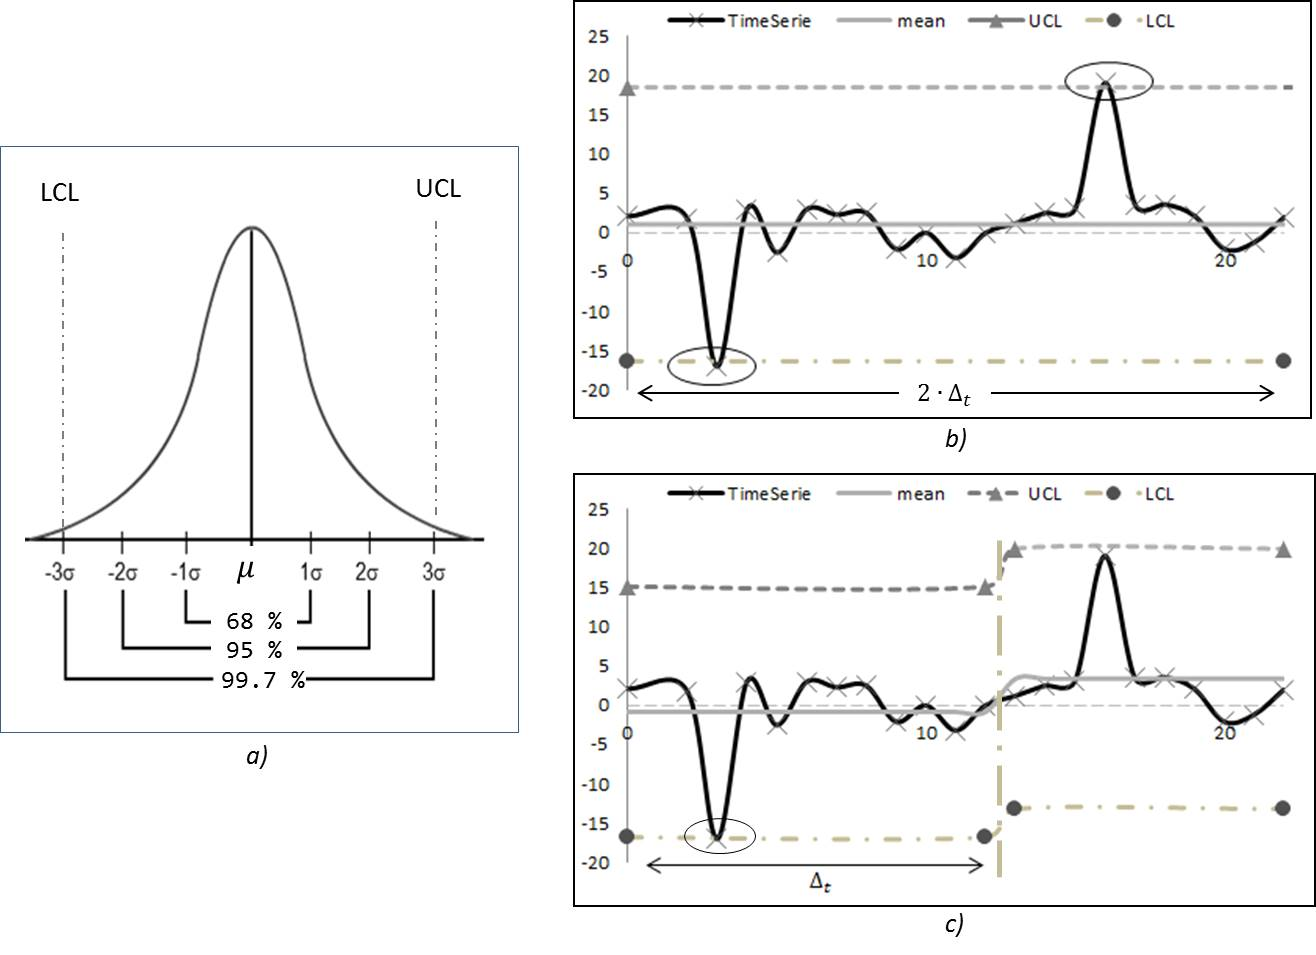
\includegraphics[scale=0.5]{Figures/Six_sigma_example.jpg}
  \caption{\textit{a)} \textbf{The 3$\sigma$'s rule}: There is a 99.7\% probability that the variable values belong to the interval $[LCL,UCL]$. \textit{b)} Six sigma approach for a time series with fixed LCL and UCL limits. Two spotted values (in the ellipse) are considered as outlier values. \textit{c)} Six Sigma approach with a windowing of $\Delta t$ size. The LCL and UCL limits are not fixed and change according to the values inside of the window.  }
  \label{fig:six_sigma}
\end{figure}

In Figure \ref{fig:six_sigma}{\color{red} .\textit{b)}}, one can observe that the $6\sigma$'s approach detects two outlier values for a window of size $2\Delta_t$, while in Figure \ref{fig:six_sigma}{\color{red} .\textit{c)}}, the same approach for a window of size $\Delta_t$ only detects one outlier value in the first window and the other, in the second window, is not detected. We observe in the experiments that the window size affects the detection of outlier values. We notice that the bigger the window is, the more chance there is to detect general outliers, but in contrast, the chance of detecting local outliers is low. We also observe that the smaller the windows is, the less general outliers we can detect. Therefore, having a good definition of the window size is critical for this approach.


\paragraph{Percentile analysis approach}

shows the use of percentile analysis for spotting
outlier values (marked inside the ellipses). This proposed approach determines the LoL and
UpL limits by a linear regression over extreme selected (or rather “selected extreme...”?) percentiles. In this example, we select



Figure \ref{fig:percentile}{\color{red} .\textit{c)}} 
shows the use of percentile analysis for spotting 
outlier values (marked inside the ellipses). This proposed approach determines the \textit{LoL} and \textit{UpL} limits by a linear regression over selected extreme percentiles. In this example, we select the percentiles $\mathbf{P}_l = [P_{5}, P_{10}, P_{15}, P_{20}, P_{25}]$ for the $LoL$ limit, and the percentiles $\mathbf{P}_u = [P_{75},P_{80},P_{85},P_{90},P_{95}]$ for the $UpL$ limit. Two trends are defined using the mentioned percentiles: 
\begin{itemize}
\item[•] The $up\_le$ trend conformed by $up\_le(x) = \mathbf{P}_u$ and $x=[0.75, 0.8, 0.85, 0.9, 0.95]$.
\item[•] The $lo\_le$ trend conformed by $lo\_le(x) = \mathbf{P}_l$ and $x=[0.05, 0.1, 0.15, 0.2, 0.25]$.
\end{itemize}

When we apply a linear regression over each trend, we find the predicted values for the points $x= 1 \to up\_le(x)$ and $x = 0 \to lo\_le(x)$. These values define the $UpL$ and $LoL$ limits respectively. These can be observed in Figure \ref{fig:percentile}{\color{red} .\textit{b)}} as $up\_le$ and $lo\_le$. Finally, we assume that if there are outlier values (using amplitude as a criteria), they would not follow the linear trend and they would be either in the $5^{th}$ percentile or the $95-100^{th}$ percentile.    

\begin{figure}[h!]
  \vspace{0.5em} %better style
  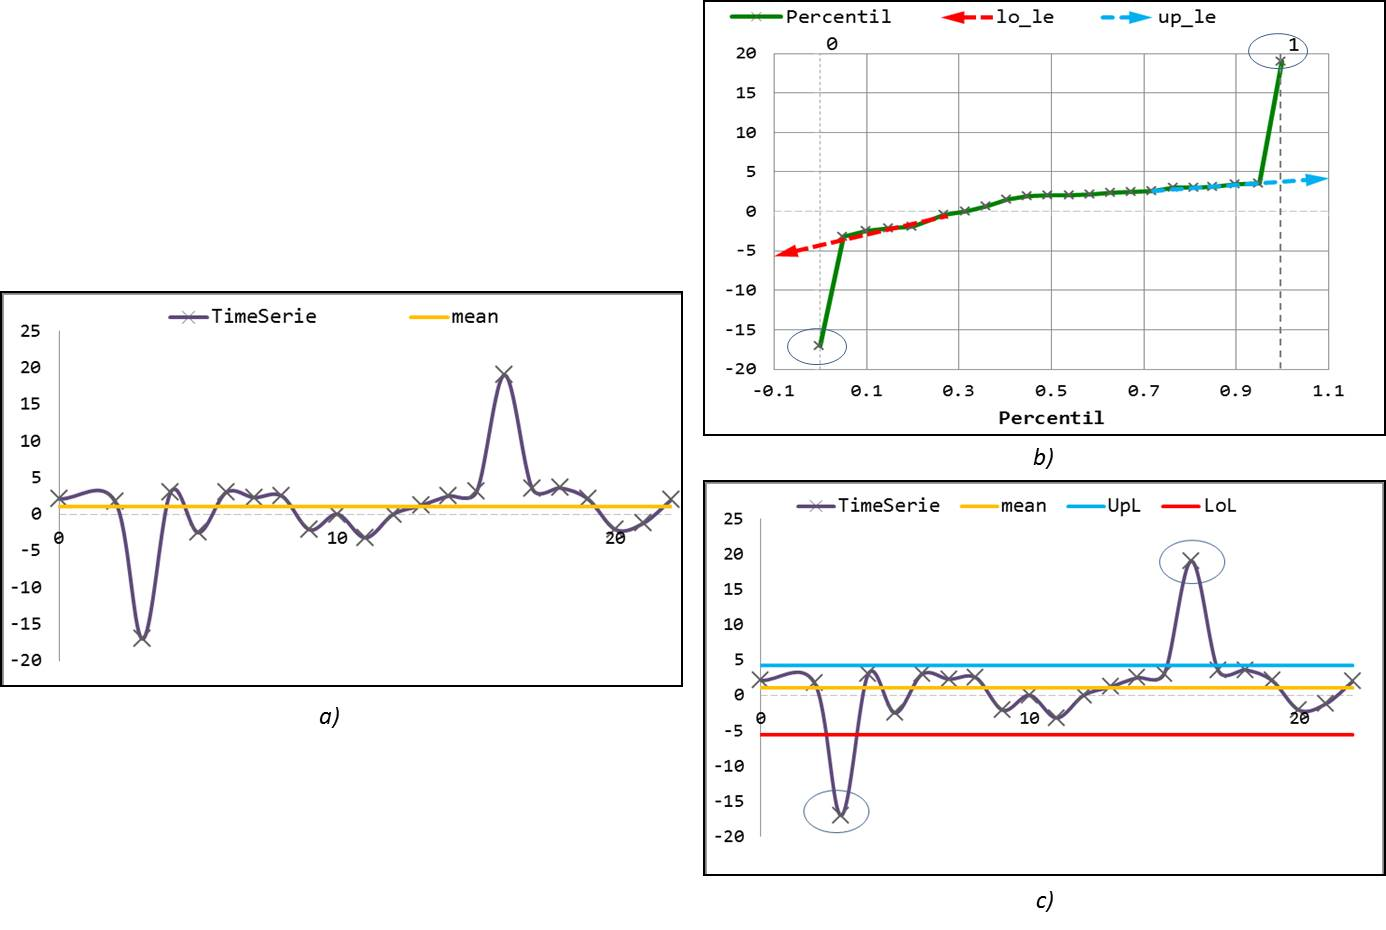
\includegraphics[scale=0.5]{Figures/percentil_example.jpg}
  \caption{\textit{a)} Simple time series, similar to Figure \ref{fig:six_sigma}. \textit{b)} Percentile curve of the time series. Trends \textit{lo\_le} and \textit{up\_le} are the linear regression of the extreme percentile values.  \textit{c)}
The percentile analysis approach detects two outlier values (in the ellipse), these values do not belong to the interval  
$[LoL, UpL]$.}
  \label{fig:percentile}
\end{figure}

In contrast to the six sigma approach, note that percentile analysis does not have symmetric limits to the mean. Observe how the $UpL$ and $LoL$ are not symmetric to the mean $\mu$ in figure \ref{fig:percentile}{\color{red} .\textit{c)}}. This property allows the use of this approach for distributions that are not necessarily Gaussian.


\begin{figure}[h!]
  \vspace{0.5em} %better style
  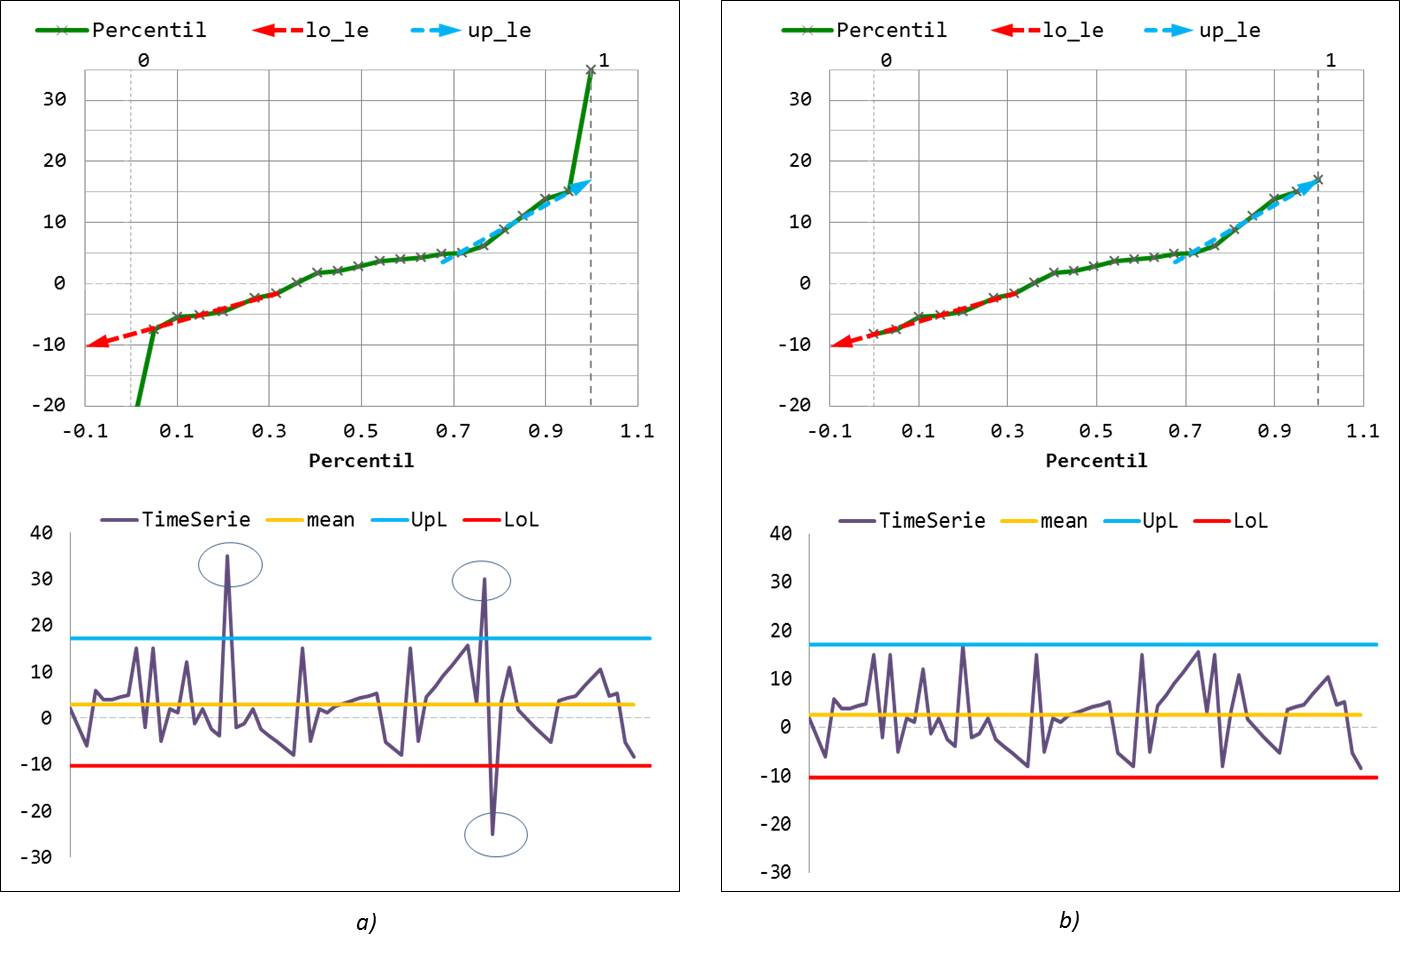
\includegraphics[scale=0.5]{Figures/percentil_example_2.jpg}
  \caption{\textit{a)} Three outliers detected using the percentile analysis approach. \textit{b)} The same time series presented without the three detected outliers.}  
  \label{fig:percentile2}
\end{figure}

To exemplify the behavior of the percentile analysis, observe Figure \ref{fig:percentile2} where any value outside the interval $[LoL, UpL]$ is detected as outlier. 

\subsubsection{Comparison between six sigma and percentile analysis}
To evaluate both approaches, we perform several experiments \footnote{The complete set of experiments are included as digital annex in \textit{/Thesis\_project/iPythonBooks/Outlier\_detection}} over theoretical signals where we define the limits of the variable. The random variable is defined by $2A \cdot$ $np.random.rand(n,1)$ $- A$ \footnote{Create an array of the given shape and populate it with random samples from a uniform distribution over [0, 1)}, therefore the variable is limited in the range $[-A, A]$. We introduce outliers on purpose, to know if both approaches detect these outliers. Figure \ref{fig:comparison} shows in \textbf{a)} the random signal in range [-10, 10] with added outilers, and \textbf{b)} the detection of outliers by using both approaches.    


\begin{figure}[h!]
  \vspace{0.5em} %better style
  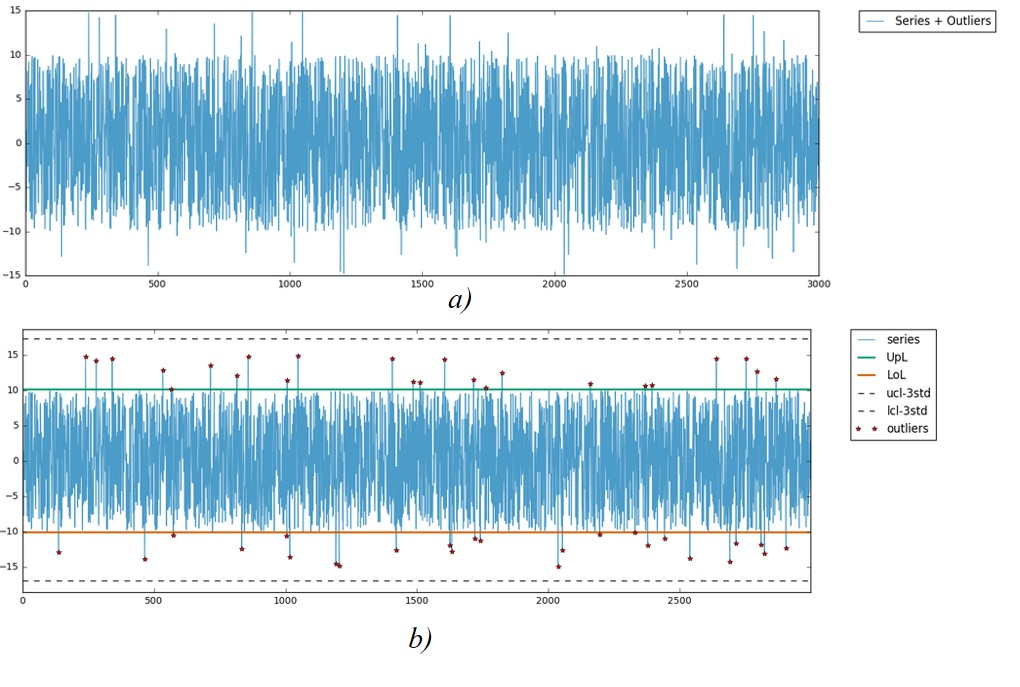
\includegraphics[scale=0.5]{Figures/test.jpg}
  \caption{\textit{a)}A random signal with range of [-10, 10] with added outliers.  \textit{b)} Detection of outliers by using six sigma and percentile analysis approach.}  
  \label{fig:comparison}
\end{figure}

One observe how the limits of the six sigma approach (i.e. ucl-3std and lcl-3std) do not detect any outlier (i.e. $0\%$) while the percentile approach detects 100\% of them. In the following experiment in figure \ref{fig:test2},we tested the quantity of outliers that this approach can detect with an accuracy greater than 95\%. We include the results of six sigma approach to make comparison between the two approaches. The tested time series has length of 3000, and one observes the detection precision  decreases less than 95\% when the original time series contains more than 300 inserted outliers.

  
\begin{figure}[h!]
  \vspace{0.5em} %better style
  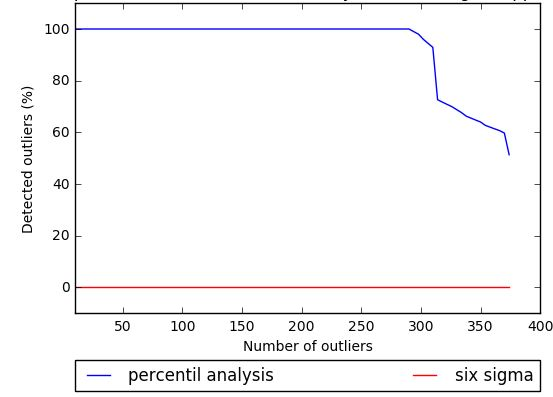
\includegraphics[scale=0.5]{Figures/test2.jpg}
  \caption{Testing the number of outliers that percentile analysis and six sigma approach can detect.}  
  \label{fig:test2}
\end{figure}

This happens because the extreme values begin to represent more than 10\% of the total points of the series. Are these points part of the process?. Figure \ref{fig:test3} shows this situation. 

\begin{figure}[h!]
  \vspace{0.5em} %better style
  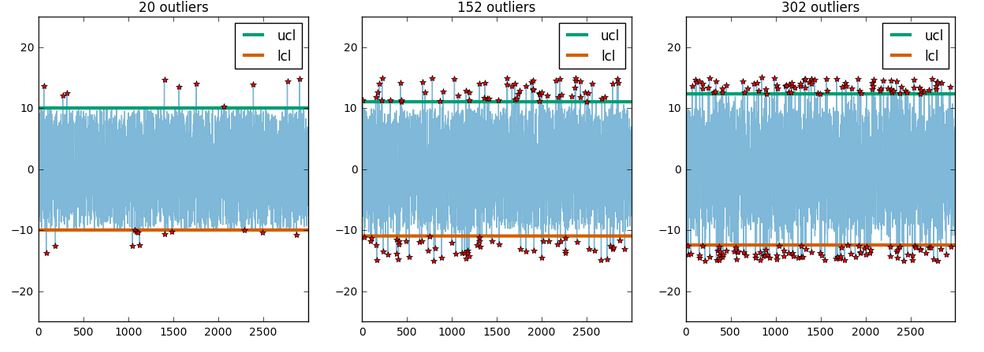
\includegraphics[scale=0.5]{Figures/test3.jpg}
  \caption{Percentile analysis approach spotting outliers.}  
  \label{fig:test3}
\end{figure}

We use the percentile analysis to depurate the time series from values that do not correspond to the underlying process of the variable. This is important because outlier values could create havoc in the training process, visualization of results and other further steps. For example, the non convergence of the tuning parameters of the model during the training process. \footnote{We save the detected values of this approach in collection: \textit{detection outlier}. Script: \textit{1. detection\_using\_quartiles.py}}. The six sigma approach is used as well when we apply the SAX process according to section \ref{comparison_sax_hmm}. Table \ref{tab:six_perc} shows the number of points that were detected as outliers for a set of variables. One observes that each approach has different results for each particular variable. We observe that the percentile analysis approach has best detected outliers, since there is no assumption of a Gaussian distribution of the time series as \textit{six-sigma} does.       


\begin{table}[]
\centering
\caption{Number of points (individual measurements) spotted as outliers.}
\label{tab:six_perc}
\tiny
\begin{tabular}{l|l|l|}
\cline{2-3}
                                                 & \multicolumn{2}{c|}{Number of detected points} \\ \hline
\multicolumn{1}{|l|}{Variable}                   & \# Percentil Analysis      & \# Six Sigma      \\ \hline
\multicolumn{1}{|l|}{V004\_vent01\_hum\_out}     & 148                        & 362               \\ \hline
\multicolumn{1}{|l|}{V023\_vent02\_temp\_out}    & 105                        & 279               \\ \hline
\multicolumn{1}{|l|}{V005\_vent01\_CO2}          & 114                        & 473               \\ \hline
\multicolumn{1}{|l|}{V022\_vent02\_CO2}          & 141                        & 474               \\ \hline
\multicolumn{1}{|l|}{V006\_vent01\_temp\_out}    & 87                         & 264               \\ \hline
\multicolumn{1}{|l|}{V012\_vent01\_temp\_in}     & 294                        & 531               \\ \hline
\multicolumn{1}{|l|}{V021\_vent02\_hum\_out}     & 193                        & 403               \\ \hline
\multicolumn{1}{|l|}{V029\_vent02\_temp\_in}     & 324                        & 604               \\ \hline
\multicolumn{1}{|l|}{V037\_tabs\_cold\_SW}       & 87                         & 152               \\ \hline
\multicolumn{1}{|l|}{V074\_tabs\_warm\_NO}       & 310                        & 280               \\ \hline
\multicolumn{1}{|l|}{V075\_tabs\_cold\_NO}       & 164                        & 132               \\ \hline
\multicolumn{1}{|l|}{V099\_blinds\_height\_N\_o} & 35                         & 13                \\ \hline
\multicolumn{1}{|l|}{V102\_blinds\_height\_N\_i} & 33                         & 13                \\ \hline
\multicolumn{1}{|l|}{V105\_blinds\_height\_O\_o} & 54                         & 17                \\ \hline
\multicolumn{1}{|l|}{V108\_blinds\_height\_O\_i} & 34                         & 12                \\ \hline
\multicolumn{1}{|l|}{V111\_blinds\_height\_S\_o} & 48                         & 16                \\ \hline
\multicolumn{1}{|l|}{V112\_blinds\_angle\_S\_o}  & 30                         & 12                \\ \hline
\multicolumn{1}{|l|}{V114\_blinds\_height\_S\_i} & 50                         & 14                \\ \hline
\multicolumn{1}{|l|}{V115\_blinds\_angle\_S\_i}  & 35                         & 10                \\ \hline
\multicolumn{1}{|l|}{V117\_blinds\_height\_W\_o} & 26                         & 11                \\ \hline
\multicolumn{1}{|l|}{V118\_blinds\_angle\_W\_o}  & 25                         & 11                \\ \hline
\multicolumn{1}{|l|}{V120\_blinds\_height\_W\_i} & 38                         & 12                \\ \hline
\multicolumn{1}{|l|}{V121\_blinds\_angle\_W\_i}  & 39                         & 11                \\ \hline
\end{tabular}
\end{table}




\section{Feature Selection}
\label{sec:feature_selection}

This module assists the selection of features for the creation of multivariate samples as it was explained in section \ref{sec:MVA}. We want to choose the best features from different variables such that one sample can express information in a more high level, making more robust and integral our proposed models. This is the approach of the \textit{GaHMM seasonal} model that is explained in section \ref{sec:seasonal_model}. One common approach to feature selection is the use of the Kullback–Leibler distance, this approach allows the measure of information when one uses an arbitrary feature. We borrowed and adapted the concepts that are presented in (\citeauthor{eguchi2006interpreting}, 2006) \cite{eguchi2006interpreting} to explain the feature selection that was performed in this study. If we let $P$ and $Q$ be two probability distributions of one feature $x$ over two different clusters of data. Then let $p(x)$ and $q(x)$ be their respective probability functions. The Kullback–Leibler distance is thus defined by:

\begin{equation}
D(P,Q) = \int p(x) log 	\dfrac{p(x)}{q(x)} dx
\end{equation}

Two basic properties of D can be observed from this formula: 
\begin{itemize}
\item[a.] non-negativity $D(Q,P) \geq 0$, and a especial case: if $P == Q$ then $D(Q,P)=0$
\item[b.] asymmetry $D(P,Q) \neq D(Q,P)$
\end{itemize}
Since this distance is asymmetry, it is normal practice to use the symmetric K–L distance (also known as J-distance) \cite{coetzee2005correcting}: 

\begin{equation}
J(p,q) = D(p,q) + D(q,p)
\label{J_distance}
\end{equation}

It follows then, that if $J(p,q) = 0$ the two clusters characterized by the feature $x$ are similar. Stated in another way, the two clusters should be a single cluster (or a feature $x$ does not provide
any information helpful to the discrimination of these two groups
). In contrast, if $J(p,q)$ is high then surely the feature $x$ describes two different clusters. Thus, one is interested in finding the features that return a high J value on latent clusters. This selection can be done by sophisticated and robust methods (\citeauthor{sui2013information}, 2013 \cite{sui2013information}). However, this work uses a simplified version for feature
selection, since we are only interested in having an approximate ranking of features, due to the evaluation process for GaHMM scoring the clustering quality of each model, so then we can be sure that the feature selection was good. The final objective of our proposition \footnote{Script \textit{2.entropy\_calculation.py} implements this proposition.} is a collection of JSON documents where one can rank the
features from the highest "gain of information" until the lowest one. This ranked list of feature is created by the following steps (see figure \ref{fig:schema} to illustrate the process):   

\begin{itemize}
\item[1] Features are calculated in a daily fashion using the script \textit{2.statistics daily.py}. The feature data space (i.e. daily feature collection) is created according to the feature list in annex \ref{tab:feature_list}.
\item[2] Random groups of data in the feature space are created. In our case, 7 groups of data were created by using the weekday name label \footnote{This choice is arbitrary. It was done because we observed that variables like $CO_2$, temperature and others change between working days and weekends. Therefore it was considered convenient to create the random clusters by using the names of the day. Other ways to create random groups can also be done.}.
\item[3] Chose one feature from the feature list and perform the K-L distance $J(p,q)$ over all the created groups in a pairwise fashion. Save the best K-L distance into the JSON document collection \textit{'feature selection'}.
\item[4] Order features according to the best J value. (i.e. ranked list).   
\end{itemize}

\begin{figure}[h!]
  \vspace{0.5em} %better style
  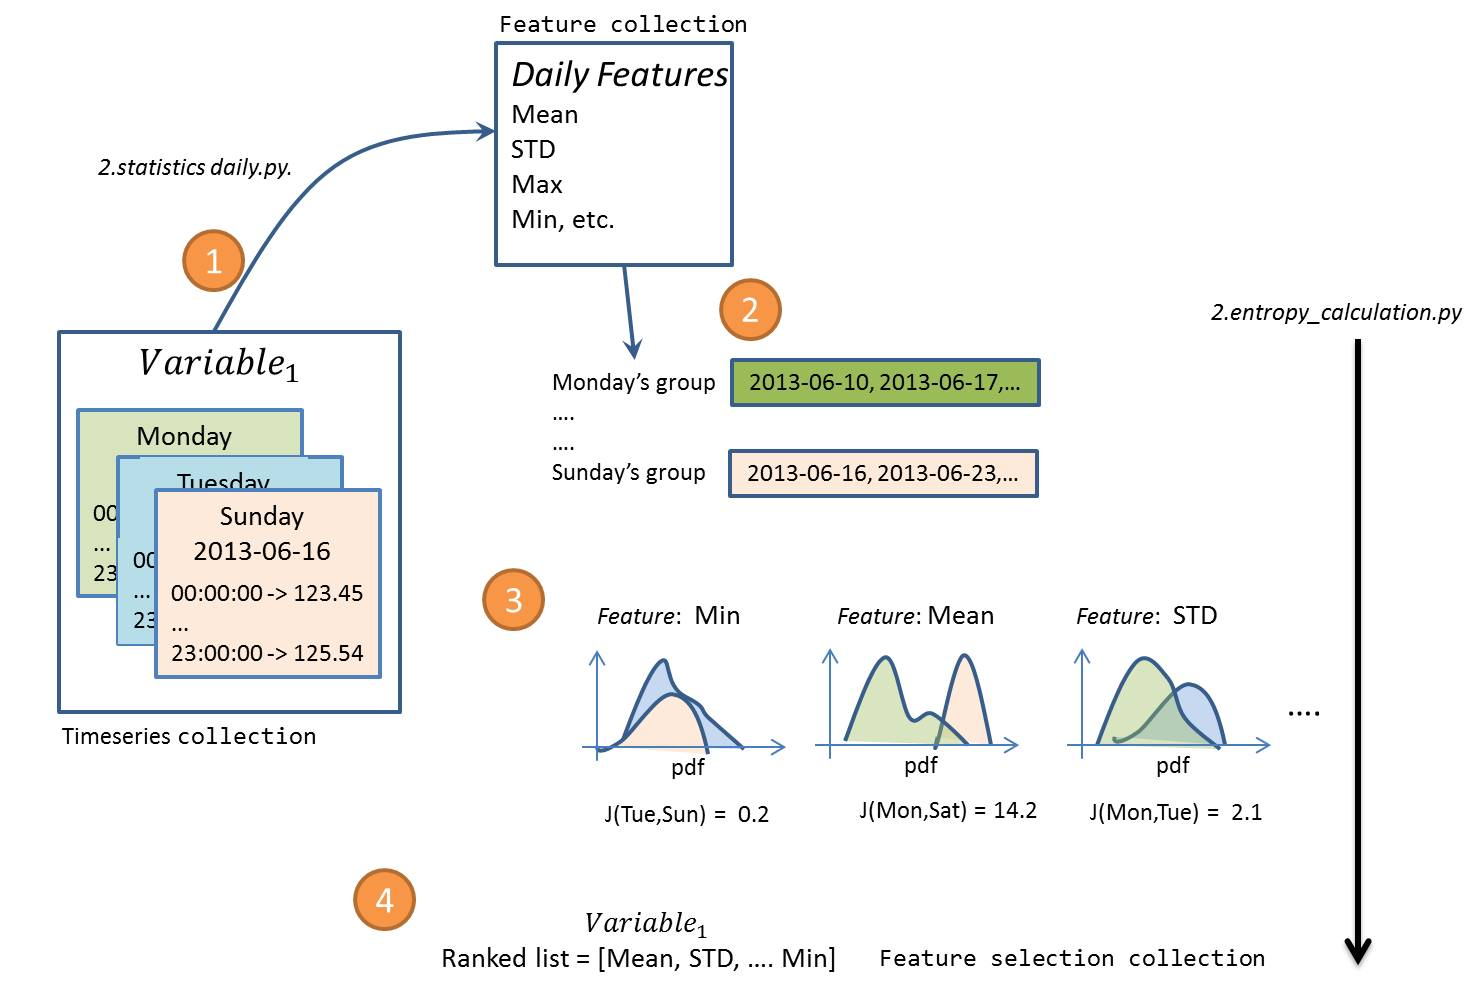
\includegraphics[scale=0.5]{Figures/feature_selection.jpg}
  \caption{Schema of the implemented feature selection}
  \label{fig:schema}
\end{figure}


By always conserving the same random groups for each interaction, it is possible to measure (approximately) the gain of information that each feature provides. Other analyses like the correlation between features can be done \cite{sui2013information}, but this is outside of the scope of this study. One can see that each variable (e.g. $CO_2$, humidity, temperature, etc.) has its own ranked list (i.e. some features that are important for a set of variable $V_1$, are less important for another set of variable $V_2$). Since we keep an invariable definition of the random groups, at the end, one can obtain a ranking of the features according his respective gain of information.


\subsubsection{Ripple Factor}
\label{sec:ripple}

We calculate 18 features in daily fashion for each variable, the complete list of features are in annex \ref{tab:feature_list}. We propose one feature that help us to gain information for the seasonal model explained in section \ref{sec:seasonal_model}. Here, we explain its concept: Given a time series of length $N$, a new feature called ripple factor captures the shape of the trend that crosses the mean $\mu_x$ of the series. The feature has three key values to converge: 
\begin{itemize}
\item[a)] The feature converges to 1 when at most points of the time series are above the mean.
\item[b)] The feature converges to 0, crossing the mean on many occasions. 
\item[c)] The feature converges to -1 when most of the point of the time series are below the mean.
\end{itemize}

This behavior is shown in figure \ref{fig:rf_ex1}. To achieve the previous description, we use a common ratio (i.e. 1/N) for all the points that belong to the series, and create a power series that maps the position of each series point $\textbf{p}$ to the exponent of each term according to the condition $\mathscr{C}_f$. In this way, all the points that are above the mean are used to form the term $A_b$ and the rest of the points are used for the term $B_e$. Finally, the difference between these two terms divided by the size of the series is the mathematical definition of our feature. The condition $\mathscr{C}_f$, the range and mathematical definition of the proposed feature are specified in equation \ref{ripple_factor}.    

\begin{figure}[h!]
  \vspace{0.5em} %better style
  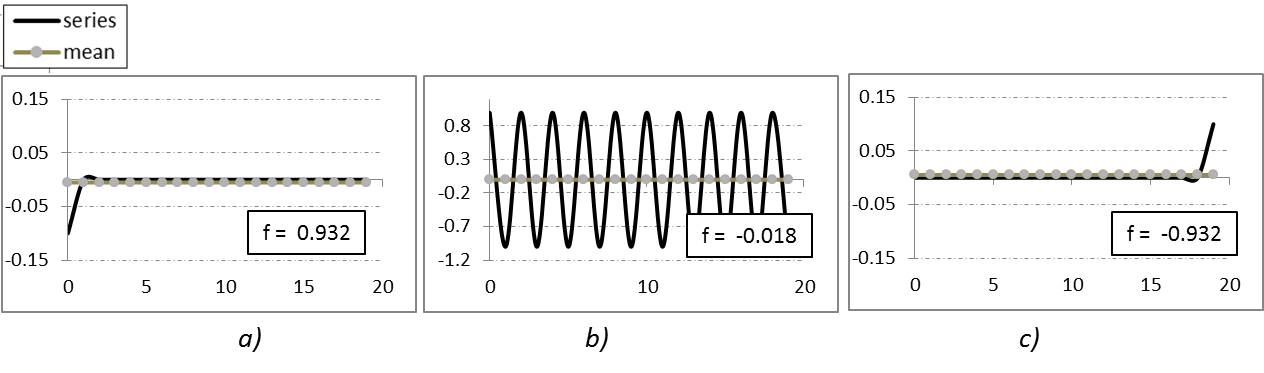
\includegraphics[scale=0.7]{Figures/Example_1_rf.jpg}
  \caption{Behavior of Ripple Factor feature}
  \label{fig:rf_ex1}
\end{figure}


\begin{equation}
\begin{array}{lcl}
\text{Time serie}			&:& X(n) = [x_0, x_1, x_2, ..., x_p], \quad |X| = N \\ \\
\text{Feature range} 		&:& \mathscr{R}_f \{ {X(n)}\} \in (-1, 1), \quad 
								\mathscr{R}_f \{ {X(n)}\} \in \mathbb{R}^+ \\ \\
\text{Feature condition}	&:& \mathscr{C}_f \{ {X}\} = \begin{cases}  
				A_b = \mathlarger{\sum_{x_p >= \mu_x} 2^{\ p \frac{1}{N}}}, & \forall p \in [0,N-1] \\ \\  											B_e = \mathlarger{\sum_{x_p < \mu_x} 2^{\ p  \frac{1}{N}}}, & \forall p \in [0,N-1] 			
							\end{cases} \\ \\
\text{Feature definition}	&:& \mathscr{R}_f \{ {y(n)}\} = ln(2) \cdot \dfrac{A_b - B_e }{N}  							
\end{array}
\label{ripple_factor}
\end{equation}

The limits of this feature are found when either $A_b$ or $B_e$ is equal to zero (but not simultaneously). For the upper limit, this occurs when all the points are above or equal to the mean. Figure \ref{fig:ripple_limits} shows how the limits behave according to the size of the series. Furthermore, we show in equation \ref{limit_cal} the upper and lower limit of this feature.

\begin{figure}[h!]
  \vspace{0.5em} %better style
  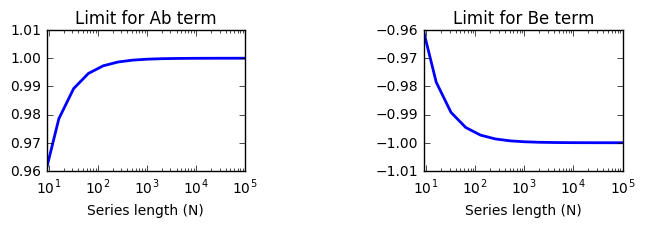
\includegraphics[scale=0.8]{Figures/limits_ripple_feature.jpg}
  \caption{Limits for the Ripple Factor feature according to the length of the time series.}
  \label{fig:ripple_limits}
\end{figure}


\begin{equation}
\begin{array}{lcl}
\text{Upper limit when $B_e = 0$} &:& \mathlarger{\lim_{N\to\infty} ln(2) \cdot \dfrac{A_b - B_e }{N} 
                                = ln(2) \cdot \lim_{N\to\infty} \dfrac{ \mathlarger{\sum_{p=0}^{N-1} \ 2^{\ p \frac{1}{N}} }}{N}}\\ \\
                              &:& \mathlarger{ ln(2) \cdot \lim_{N\to\infty} \dfrac{1}{ N (2^{\ \frac{1}{N}}-1)} = 1 }  \\ 	
                              
\text{Lower limit when $A_b = 0$} &:& \mathlarger{\lim_{N\to\infty} ln(2) \cdot \dfrac{A_b - B_e }{N} 
                                = -ln(2) \cdot \lim_{N\to\infty} \dfrac{ \mathlarger{-\sum_{p=0}^{N-1} \ 2^{\ p \frac{1}{N}} }}{N}}\\ \\
                              &:& \mathlarger{-ln(2) \cdot \lim_{N\to\infty} \dfrac{1}{ N (2^{\ \frac{1}{N}}-1)} = -1 } 						
\end{array}
\label{limit_cal}
\end{equation}

The following part discusses several examples that use this feature. We propose comparable examples where the mean is equal to zero in all the cases. The capacity of the ripple factor to discriminate time series that have similar statistics is appreciated in figure \ref{fig:rf_ex2}. The three time series have the same mean, variance, percentiles, and maximum and minimum value, but the ripple factor for each one is different, so that, we can discriminate for example a sine signal from a cosine signal. 

\begin{figure}[h!]
  \vspace{0.5em} %better style
  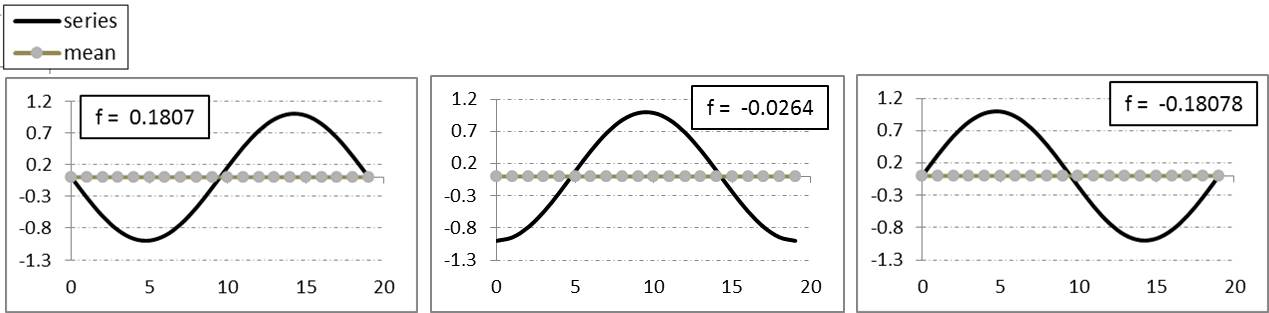
\includegraphics[scale=0.7]{Figures/Example_2_rf.jpg}
  \caption{Ripple factor for sine and cosine signal.}
  \label{fig:rf_ex2}
\end{figure}

In figure \ref{fig:rf_ex3}, we appreciate how this feature changes depending on the shape of each particular signal. The examples show how this feature changes as soon as the oscillations approach the mean. The closer the oscillations are to the mean, the nearer to zero the feature is. \\

\begin{figure}[h!]
  \vspace{0.5em} %better style
  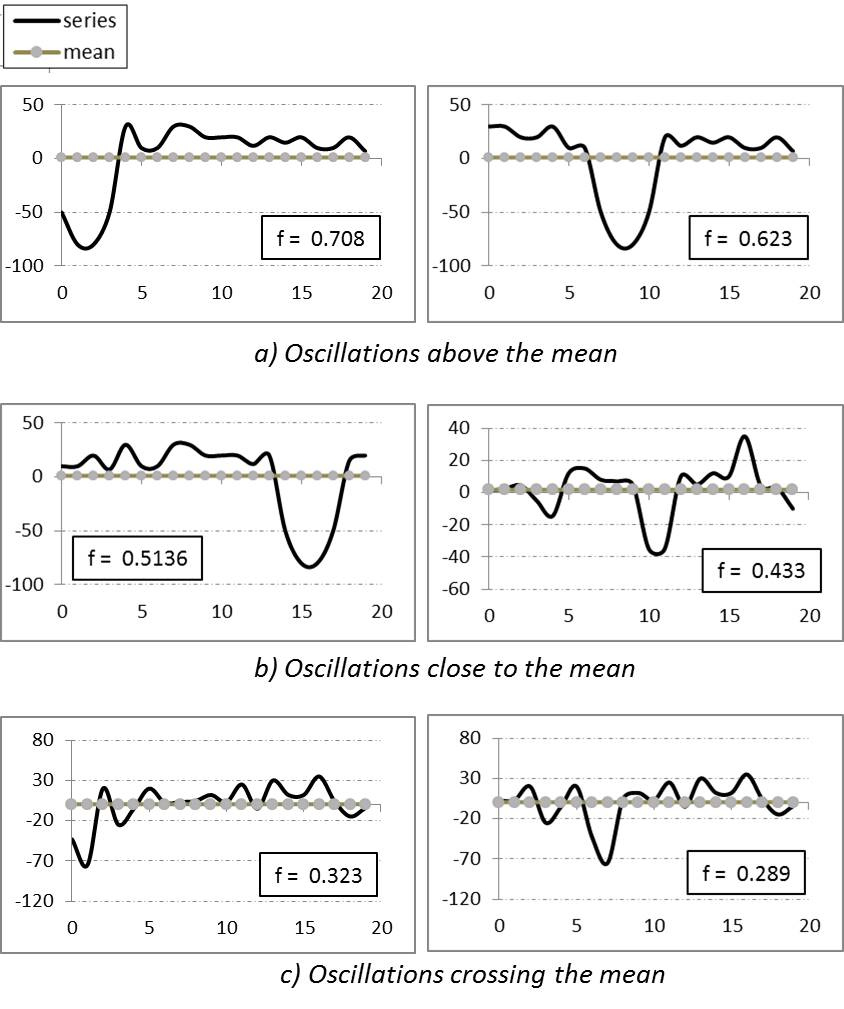
\includegraphics[scale=0.7]{Figures/Example_3_rf.jpg}
  \caption{Ripple factor for sine and cosine final.}
  \label{fig:rf_ex3}
\end{figure}


\textit{Extension of the ripple factor feature:} \\

The last behavior explained in figure \ref{fig:rf_ex3} allows to extend the concept of the ripple factor to one that is most general. If we change the definition of the feature condition $\mathscr{C}_f$, we can substitute the parameter of comparison (in the original definition $\mu_x$) for any other numeric value $v \in \mathbb{R}$. This change is useful when for some reason we need to know whether or not most of the
oscillations are close to the value $v$ \\


\textit{Discussion of the Ripple Factor:} \\
 
As we see in figure \ref{fig:ripple_limits} the feature is sensitive to the length of the series. Nevertheless, for this study the feature was calculated using a fixed window of one day (i.e. sub-sequences of same size), therefore the limits are well defined. To know how much these limits differ, we consider a time series of size $N=10$ and one of size $N=50$. Their limits are $0.965$ and $0.993$ respectively and the difference is only 0.028. To know whether this difference is significant, an evaluation must be done. The mentioned evaluation goes beyond the purposes of this study and we only use this feature because the length of sub-sequences is fixed (therefore the limits are well defined) and because using the Kullback–Leibler divergence, this feature obtains a good gain of information being selected for the \textit{GaHMM-seasonal} profile, explained in section \ref{sec:seasonal_model}. \\

Another relevant aspect of this feature is the fact that it does not depend on the amplitude of the treated signal. This fact allows the signal to be amplified or reduced without changing the ripple factor. This can be an advantage when the shape of the series is an important characteristic to analyze. Finally, this feature is complementary to other statistics such as the the mean, standard deviation and others, but not a substitute for them.




\section{GaHMM Modeling}
\label{modeling}

Hmmlearn \cite{gahmm_manual} \footnote{\url{http://hmmlearn.readthedocs.io/en/stable/}} is the python library used in this project. We use the internal methods that this library offers in order to perform the training process. We recall here the training process that was explained in section \ref{sec:problems}, and we add information about the employed library. 


\begin{itemize}
\item Learning/ training process: The HMM model is fitted with the observed samples $\mathbb{O} = (O_1, O_T)$. The definition of the observed samples is very important since it defines the kind of HMM to use. Each proposed model define the samples according to the underlying problem that each model wants to solve. In all the cases we use a \textit{GaHMM} model since we use sequential continuous values. The definition of the observed samples are explained in each model. The library method to use for the training process is called: \textbf{fit} method \cite{gahmm_manual}, this implements the solution that was explained in section \ref{sec:learning_HMM}.
\item Evaluation process: For evaluation purposes, the log probability of $P(\mathbb{O} |\mathbb{S}, \lambda)$ (i.e. equation \ref{independence_ass}) is used to select the best trained model. The model that fits the best the parameters of $\lambda$ is the one who has the greatest probability. The library method that calculates $P(\mathbb{O} |\mathbb{S}, \lambda)$ is the \textbf{score} method using the forward/backward algorithm (section \ref{sec:evaluation_HMM}).    
\item Decoding process: When one obtain the best model, there is a perfect matching between the observed samples $\mathbb{O}$ and the sequences of states $\mathbb{S}$. One says that each hidden state $S_k$ emits one sample $O_i$. To know the likely sequence of hidden states the \textbf{predict} method solves the decoding problem by using Viterbi algorithm. (section \ref{sec:decoding_HMM}).  
\end{itemize}

\subsection{GaHMM Training process}
\label{sec:training_process}
 
The training process is done by solving the HMM evaluation problem (section \ref{sec:evaluation_HMM}). This evaluation is done by the \textit{score} method \cite{gahmm_manual}, where the log probability of $p(\mathbb{O}|\lambda)$ is calculated. The log probability has practical advantages, and is useful for finding the best trained model. This work adopts the use of the log probability of $p(\mathbb{O}|\lambda)$ for finding the best model. However, since its value is not easy to understand, this document reports probability in the interval of [0,1]. For this purpose, given that each observation could have been drawn by each every hidden state with a certain probability, this allows us to perform a time-dependent clustering task \citep{pfundstein2011hidden}. In this way, given the observed sequence $\mathbb{O} = (O_1, O_2,... O_T)$ and the correspondent sequence of hidden states $\mathbb{S} = (S_1, S_2,..., S_T)$ \footnote{Recall: There are $K$ hidden states for a HMM, therefore $\mathbb{S}$ is a permutation of $K$ values with length equal to $T$}, we calculate the average of $p(\mathbb{O}|\mathbb{S})$ as follows:

\begin{equation}
\overline{p}(\mathbb{O}|\mathbb{S}) = \dfrac{1}{T} \sum_{i=1}^{T} p(O_i | S_i)
\label{ec:average_probabilty}
\end{equation}

Where $T$ is the total number of observations, $S_i$ is the likely hidden state that emits the observation $O_i$, and $ p(O_i | S_i) \in [0,1]$ is the probability that the observed sample $O_i$ was emitted by the hidden state $S_i$. The hidden state sequence $\mathbb{S}$ that matches with the observed sequence is found by the \textbf{predict} method \cite{gahmm_manual} of the GaHMM library. It follows that the bigger the log probability is, the better the average $p(\mathbb{O}|\mathbb{S})$ is. Therefore, the equation \ref{ec:average_probabilty} shows a direct relationship with the log probability and his range is in the interval of [0,1].This is the way in which we will report
the results throughout the document.

    
\subsubsection{Cross validation process}
\label{sec:cross}

As is explained in section \ref{sec:learning_HMM}, the EM algorithm is a gradient-based optimization method that can be stuck in local optima. Hence, it is generally recommended to run several instances of the model with various initialization values, and then choose the best one. This process of training leads to problems of over-fitting in some cases. To avoid this, and to guarantee a well-trained model, the cross-validation technique is performed in most of the cases. Since our proposition deals with time series, the k-fold cross-validation technique is
not necessarily valid if we do not consider the time correspondence (\citeauthor{bergmeir2015note}, 2015) \cite{bergmeir2015note}. The traditional k-fold cross validation performs a random partitioning of the original sequence into k equal sized blocks. One inconvenient is that the samples are treated as independent sequences and not as a part of a sequence of events. Fitting the HMM with a random order of samples $O_i$ causes a poor performance of the model. Our proposed approach for cross-validation follows the indications of \citeauthor{bergmeir2015note}'s work, therefore the random selection is avoided. In short, the partial observed sequences for training $\mathbb{O}_{train}$ and testing $\mathbb{O}_{testing}$ respect the original order of the time series. Figure \ref{fig:k-fold} shows the schema for k-fold cross validation of $k=5$. 


\begin{figure}[h!]
  \vspace{0.5em} %better style
  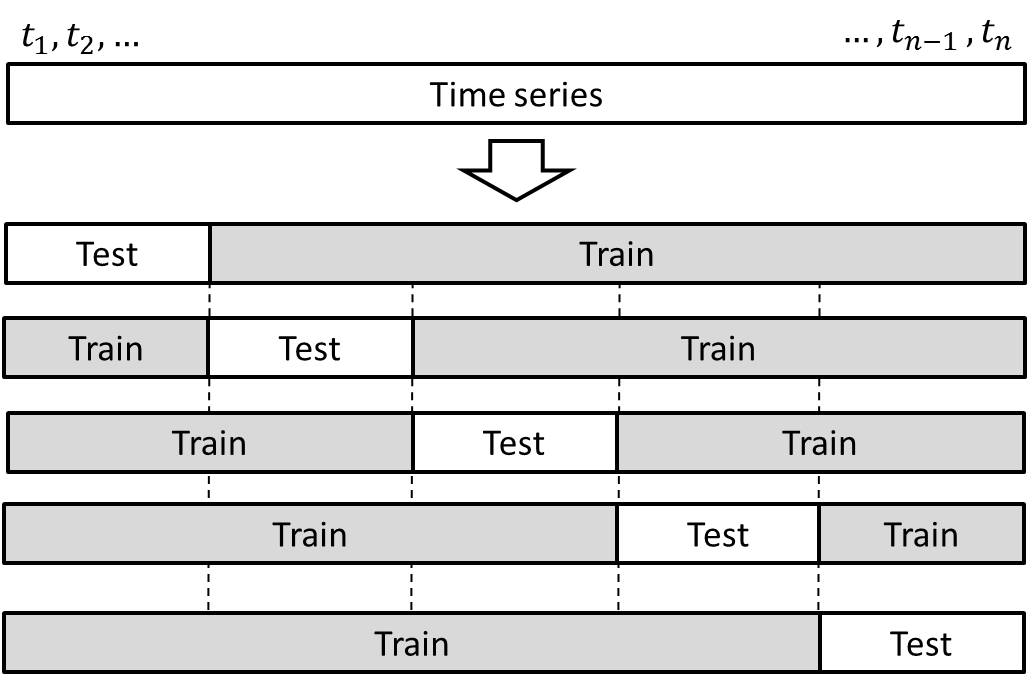
\includegraphics[scale=0.45]{Figures/k-fold.jpg}
  \caption{k-fold cross validation with $k=5$. Note that the order of the time series is not altered, no random selection is done.}
  \label{fig:k-fold}
\end{figure}


\subsubsection{Fixing parameters of GaHMM and cross validation process}

Fortunately, the GaHMM library  \cite{gahmm_manual} proposes some parameters by default. Since the Gaussian Model implements a monitor routine for checking the internal convergence, there was no need to change the default parameters for: \textit{min\_covar, means\_prior, means\_weight, n\_iter, tol}. Nevertheless, in order to guarantee the convergence of the trained model, each hidden state uses a diagonal covariance matrix (i.e. \textit{covariance\_type= "diag"}). Additionally, as it was explained in section \ref{sec:evaluation_HMM}, Viterbi algorithm was chosen by default. The only parameter that was modified for each training round was the number of components, which is the number of hidden states to use (i.e. \textit{n\_components} parameter). Regarding the cross validation process, we found by doing experiments that select $k$ in the interval of [10, 15] is a good choice. If $k < 10$, the final clusters tend to be mixed, while $k > 20$, the over-fitting effect is evident.  


\paragraph{Scripts for training}
Two python scripts were created for training the three different models explained in section \ref{implemented}. Table \ref{scripts_impl} presents the context were each script is used. Details about the models are in the next section, here the structure of each training script is explained.  

Both training scripts vary the \textit{n\_components} parameter in an interval of $[n_{min}, n_{max}]$, in which $n\_components = n$ the k-fold cross validation process is executed, afterwards the best model is chosen (for us, this is called a round). At the end, the best model $M_j$ among all the rounds is picked as the final model. This process is explained in the following pseudo-codes:


\begin{table}[]
\centering
\scriptsize
\caption{Implemented scripts for training}
\label{scripts_impl}
\begin{tabular}{|l|l|l|}
\hline
\textbf{GaHMM model} & \textbf{Script}                           & \textbf{Observed sample type}                              \\ \hline
Profile              & 4.hmm\_learning\_per\_variable\_k-fold.py & Univariate sample (daily profile of the selected variable) \\ \hline
Seasonal             & 4.hmm\_learning\_k-fold.py                & Multivariate sample (features of several variables)        \\ \hline
Interactional        & 4.hmm\_learning\_k-fold.py                & Multivariate sample (linear correlation between variables) \\ \hline
\end{tabular}
\end{table}


\begin{figure}[h!]
  \vspace{0.5em} %better style
  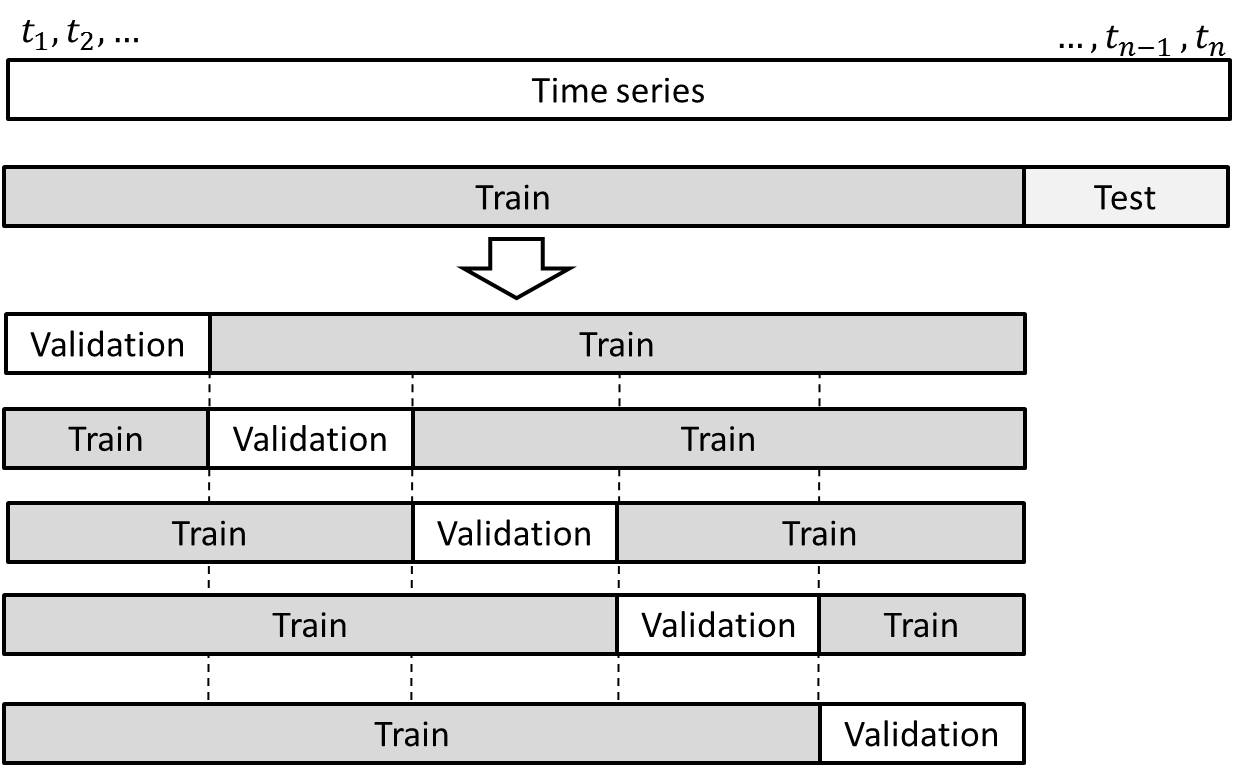
\includegraphics[scale=0.45]{Figures/k-fold-1.jpg}
  \caption{k-fold cross-validation with $k=5$ for a \textit{GaHMM} model. The testing
set is separated to be used at the end of the k-fold cross validation process (Script: \textit{4.hmm\_learning\_k-fold.py}).}
  \label{fig:k-fold-1}
\end{figure}

Pseudo-code for script \textit{4.hmm\_learning\_k-fold.py}:  

\begin{itemize}
\item[1] Extract information from the \textit{metadata} collection for the running of the corresponding training process. (i.e. variables, categories, daily vector to use, etc.)
\item[2] Establish the timeline to work with, the training set and the testing set \footnote{The testing set differs from the validation set. The testing set is a reserved part of the whole data that is used
just at the end of the whole training process. Its purpose is to test if the trained model is capable also of working on data that it has not seen before}. Here the observed sequence $\mathbb{O}$ is defined.  
\item[3] Define the minimum and maximum number of hidden states for the training process. $n \in [n_{min}, n_{max}]$. Initialize $n= n_{min}$.
\item[4] Initialize a Gaussian Hidden Markov model with $n\_components = n$.
\item[5] Perform the k-fold cross-validation over the training data set, see figure \ref{fig:k-fold-1}. At each step of the cross-validation process, the best \textit{GaHMM} model ($M_i$) is chosen by using the validation set \footnote{For this purpose, the log probability of $p(\mathbb{O}|\lambda)$ of the trained model is used.}. 
\item[6] Test the best model ($M_i$) that was found in the k-fold cross-validation process using the test set. Compare the current model ($M_i$) with the last best model ($M_j$) and elect the best model \footnote{$M_j$ is the best model to have been found among all the rounds. When $n=n_{min}$ then $M_j = M_i$. }.
\item[7] Increase the number of hidden states $n = n+1$. If $n<n_{max}$ then go to step 4, otherwise the training process is finished.  
\end{itemize}  


\begin{figure}[h!]
  \vspace{0.5em} %better style
  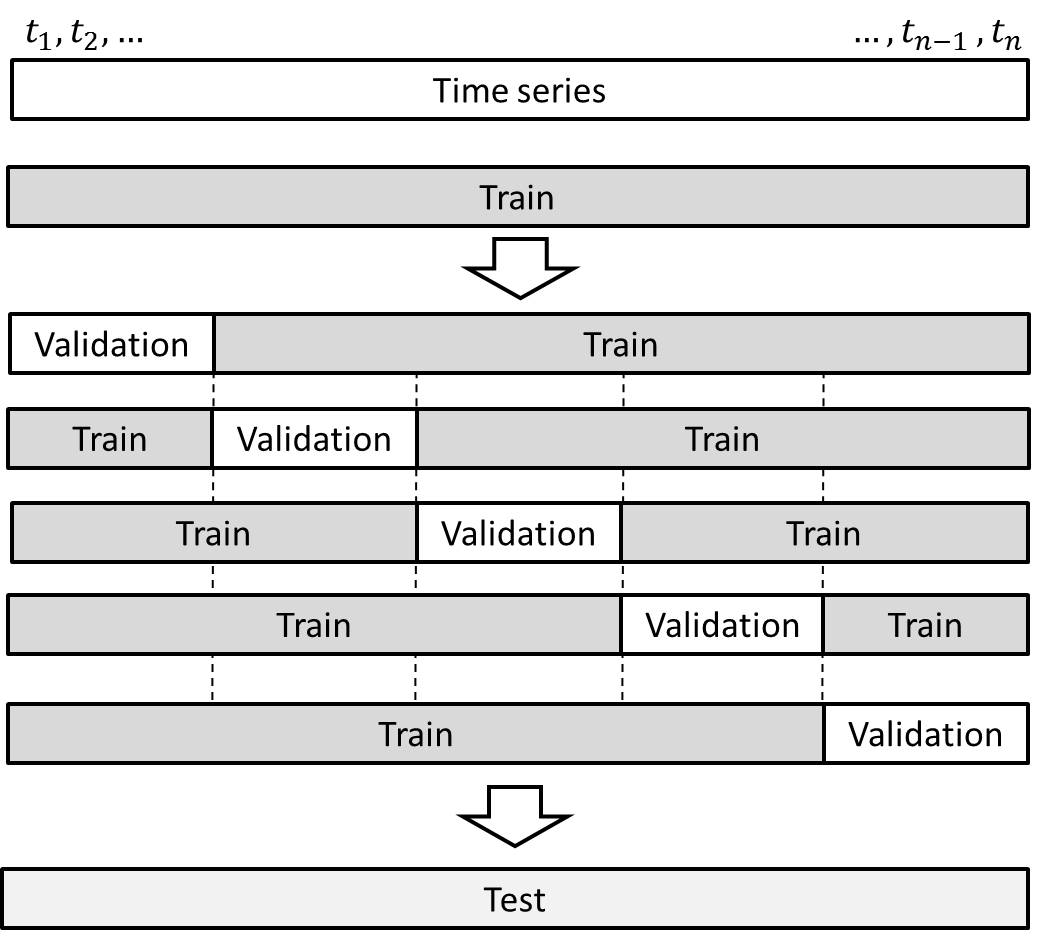
\includegraphics[scale=0.45]{Figures/k-fold-2.jpg}
  \caption{k-fold cross validation with $k=5$ for a \textit{GaHMM} model. The testing set is the entire time series. This allows the verification of the fitness of the model across the
entire time series (Script: \textit{4.hmm\_learning\_per\_variable\_k-fold.py}).}
  \label{fig:k-fold-2}
\end{figure}

Here the pseudo-code for script \textit{ 4.hmm\_learning\_per\_variable\_k-fold}: 

\begin{itemize}
\item[1] Extract information from the \textit{metadata} collection for running the correspondent training process. (i.e. variables, categories, daily vector to use, etc.)
\item[2] Establish the timeline to work with, and the training set \footnote{Since we are interested in finding all possible daily patterns across multiple years, at the end of the cross validation process, we test each model with all the available data.}. Here the observed sequence $\mathbb{O}$ is defined.   
\item[3] Define the minimum and maximum number of hidden states for the training process. $n \in [n_{min}, n_{max}]$. Initialize $n= n_{min}$.
\item[4] Initialize a Gaussian Hidden Markov model with $n\_components = n$.
\item[5] Perform the k-fold cross-validation over the training data set, see figure \ref{fig:k-fold-2}. At each step of the cross-validation process, the best \textit{GaHMM} model is chosen by using the validation set \footnote{For this purpose, the log probability of $p(\mathbb{O}|\lambda)$ of the trained model is used.}. 
\item[6] Test the best model $M_i$ that was found in the k-fold cross validation process using the test set. Compare the current model $M_i$ with the last best model $M_j$ and elect the best model.
\item[7] Increase the number of hidden states $n = n+1$. If $n<n_{max}$ then return to step 4, otherwise the training process is finished.  
\end{itemize} 

\subsection{Implemented GaHMM models}
\label{implemented}
\subsection{GaHMM - profile model}
\label{sec:profile_model}

We propose the use of the \textit{GaHMM - profile} model for performing a time-depending clustering task over a time series of interest. This implies that each variable in the multivariate building dataset has his own model. To exemplify the time-depending clustering task, we can take the time series of $CO_2$ levels of the North-East ventilation system. The time series is divided in a daily fashion, consequently 1081 observed samples were created for the whole timeline ($\approx$ 3 years). Figure \ref{fig:daily_split} shows how each sub-sequence of the entire trend (i.e. daily profile) is considered as an observed sample $O_i$.      


\begin{figure}[h!]
  \vspace{0.5em} %better style
  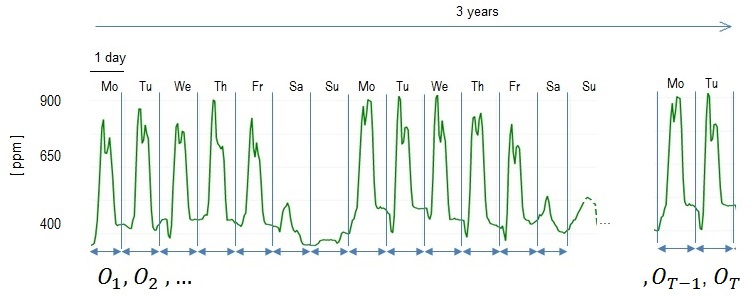
\includegraphics[scale=0.7]{Figures/split_time_series.jpg}
  \caption{ The $CO_2$ time series for the North-East ventilation system is split in a daily fashion. Each daily profile is an observed sample $O_i$.}
  \label{fig:daily_split}
\end{figure}

The observed sequence $\mathbb{O}$ is defined as a matrix of $24 \times 1081$ size. Each sample $O_i$ is a vector of length $L=24$ where each hour of the day has a corresponding value. Once the observed sequence is defined, the training process for the \textit{GaHMM - profile} is performed according to section \ref{sec:training_process} (\textit{ 4.hmm\_learning\_per\_variable\_k-fold}). The best \textit{GaHMM - profile} model is found by maximizing the likelihood of $p(\mathbb{O}|\lambda)$. At the end of the process, once the best model is found, we assume that there is a hidden state $S_k$ that is responsible for generating a sample $O_i$. In this way, we can find the best match between the sequence of hidden states $\mathbb{S}$ and the observed sequence $\mathbb{O}$. Using the Viterbi's algorithm we can discover the hidden state sequence $\mathbb{S}$ and, in this way, perform the time-depending clustering. Figure \ref{fig:daily_cluster} shows a hypothetical example where the $CO_2$ time series is disaggregated by daily profiles $O_i$ and the observed sequence is matched with the hidden state sequence $\mathbb{S} = [2,5,0,4,2,4,1,6,3,3,0,2,4,1]$. Then using the identification $ID$ of the hidden states, we can cluster days with similar daily profiles. For practical purposes, we name each cluster with the number of the associated hidden state (i.e. $ID = S_k$).  


\begin{figure}[h!]
  \vspace{0.5em} %better style
  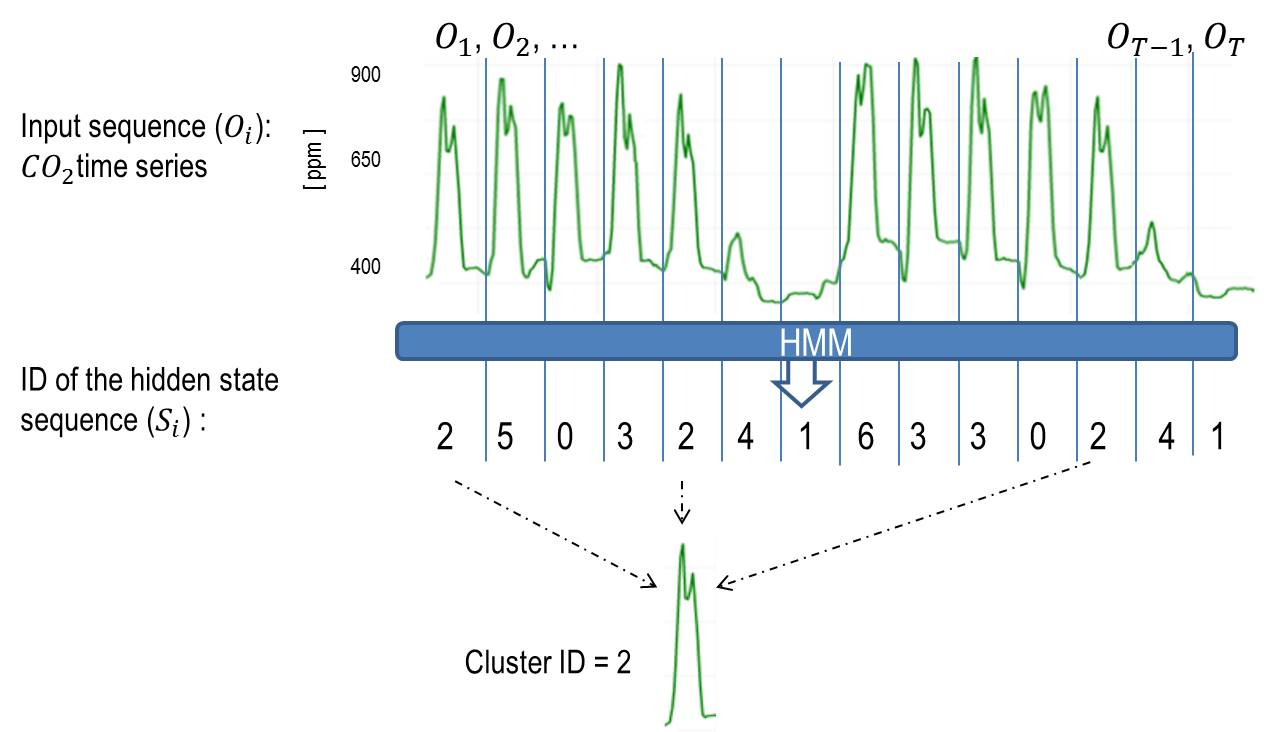
\includegraphics[scale=0.7]{Figures/sequence_explanation.jpg}
  \caption{Hypothetical example: The $CO_2$ time series is "emitted" by a $GaHMM$ model of 7 hidden states. $\mathbb{S} = [2,5,0,4,2,4,1,6,3,3,0,2,4,1]$. At the bottom-center the daily profile for cluster $ID=2$ corresponding to the hidden state $S_k=2$.}
  \label{fig:daily_cluster}
\end{figure}

The results of this model are discussed in section \ref{section:CO2_analysis} where the model is applied over the $CO_2$ time series in a case study. The quality of the cluster is reflected directly in the log probability of $p(\mathbb{O}|\lambda)$ and the average of $p(\mathbb{O}|\mathbb{S})$. However, to get a visual evaluation of the model, each cluster can be plotted out using box plots. A good cluster is one who has few (if any) outliers (i.e. fliers) outside of the whiskers. Examples of these daily profile clusters are in annex \ref{fig:candidates_profiles_NE}.


\subsection{GaHMM - seasonal model}
\label{sec:seasonal_model}

Several factors affect the way in which a building performs during the day. One of them is without a doubt, the outdoor conditions \cite{miller2015forensically, miller2015automated, djamila2017indoor}. The main purpose of this model is to cluster days according to the similarity of the outdoor conditions. In this way, we can use the information for understanding the dynamics of the building across seasons. For this purpose, the available \textbf{weather variables} (i.e. \textit{Outdoor temperature of the building, sunshine presence, precipitation and weather temperature}) are used for finding seasonal groups in the dataset. 


\paragraph{Implementation}  

A daily sample $O_i$ for this model is defined as a vector that contains selected features from the different weather variables. For practical purposes, this vector is herein called as $S_{vector}$. Features from the weather variables are calculated in a daily fashion \footnote{script \textit{2.statistics daily.py}}. Afterwards the entropy value for each feature is calculated by using the Kullback–Leibler divergence distance \footnote{Script: \textit{2.entropy\_calculation.py}} according to section \ref{sec:feature_selection}). This last value and the training process of the \textit{GaHMM} allows us to perform the feature selection in an indirect fashion. The final seasonal model uses only six features of a list of nineteen features (annex \ref{tab:feature_list}). These six selected features \footnote{The selection feature is done in an indirectly fashion by the training process, see in section \ref{sec:seasonal_evaluation}. The best model is reached by using six features among all, observe table \ref{tab:feature_gain} where the best features are in orange color} present in general, the maximum values of entropy among the list of features. Table \ref{tab:feature_gain} shows the gain of information of each individual feature, the bigger the value is, the more information we gain. This information can be retrieved from the \textit{'feature selection'} collection. In this way, each feature can be ranked according its gain of information. Thus, $F_1$ gains more information with and $F_{19}$ gains the less. In this way, from a collection of $m$ variables, a daily sample $O_i$ contains $f$ features of each variables $V$, that is:


% Please add the following required packages to your document preamble:
% \usepackage[table,xcdraw]{xcolor}
% If you use beamer only pass "xcolor=table" option, i.e. \documentclass[xcolor=table]{beamer}
\begin{table}[]
\centering
\caption{Entropy value $J$ for the \textit{weather variables}. It shows the gain of information for each variable according to section \ref{sec:feature_selection}. Definition of each feature in annex \ref{tab:feature_list}.}
\scriptsize
\label{tab:feature_gain}
\begin{tabular}{|l|l|l|l|l|l|l|l|l|lll}
\cline{1-3} \cline{5-6} \cline{8-9} \cline{11-12}
\multicolumn{1}{|c|}{\textit{\textbf{}}} & \multicolumn{2}{c|}{\cellcolor[HTML]{9AFF99}\textit{\textbf{Sunshine presence}}}                                                       & \multicolumn{1}{c|}{\textit{\textbf{}}} & \multicolumn{2}{c|}{\cellcolor[HTML]{9AFF99}\textit{\textbf{Outdoor temperature}}}                                                     & \multicolumn{1}{c|}{\textit{\textbf{}}} & \multicolumn{2}{c|}{\cellcolor[HTML]{9AFF99}\textit{\textbf{Weather Temperature}}}                                                     & \multicolumn{1}{c|}{\textit{\textbf{}}} & \multicolumn{2}{c|}{\cellcolor[HTML]{9AFF99}\textit{\textbf{Precipitation}}}                                                           \\ \cline{1-3} \cline{5-6} \cline{8-9} \cline{11-12} 
\multicolumn{1}{|c|}{\textit{\textbf{}}} & \multicolumn{1}{c|}{\cellcolor[HTML]{9AFF99}\textit{\textbf{f}}} & \multicolumn{1}{c|}{\cellcolor[HTML]{9AFF99}\textit{\textbf{J(f)}}} & \multicolumn{1}{c|}{\textit{\textbf{}}} & \multicolumn{1}{c|}{\cellcolor[HTML]{9AFF99}\textit{\textbf{f}}} & \multicolumn{1}{c|}{\cellcolor[HTML]{9AFF99}\textit{\textbf{J(f)}}} & \multicolumn{1}{c|}{\textit{\textbf{}}} & \multicolumn{1}{c|}{\cellcolor[HTML]{9AFF99}\textit{\textbf{f}}} & \multicolumn{1}{c|}{\cellcolor[HTML]{9AFF99}\textit{\textbf{J(f)}}} & \multicolumn{1}{c|}{\textit{\textbf{}}} & \multicolumn{1}{c|}{\cellcolor[HTML]{9AFF99}\textit{\textbf{f}}} & \multicolumn{1}{c|}{\cellcolor[HTML]{9AFF99}\textit{\textbf{J(f)}}} \\ \cline{1-3} \cline{5-6} \cline{8-9} \cline{11-12} 
$F_1$                                        & \cellcolor[HTML]{FFCE93}r\_factor\_st                            & \cellcolor[HTML]{FFCE93}inf                                         &                                         & \cellcolor[HTML]{FFCE93}r\_factor\_ed                            & \cellcolor[HTML]{FFCE93}1.00                                        &                                         & \cellcolor[HTML]{FFCE93}r\_factor\_ed                            & \cellcolor[HTML]{FFCE93}1.00                                        & \multicolumn{1}{l|}{}                   & \multicolumn{1}{l|}{\cellcolor[HTML]{FFCE93}max\_ed}             & \multicolumn{1}{l|}{\cellcolor[HTML]{FFCE93} inf}                       \\ \cline{1-3} \cline{5-6} \cline{8-9} \cline{11-12} 
$F_2$                                        & \cellcolor[HTML]{FFCE93}r\_factor\_ed                            & \cellcolor[HTML]{FFCE93}0.23                                        &                                         & \cellcolor[HTML]{FFCE93}r\_factor                                & \cellcolor[HTML]{FFCE93}0.51                                        &                                         & \cellcolor[HTML]{FFCE93}r\_factor                                & \cellcolor[HTML]{FFCE93}0.98                                        & \multicolumn{1}{l|}{}                   & \multicolumn{1}{l|}{\cellcolor[HTML]{FFCE93}(max-min)*std}       & \multicolumn{1}{l|}{\cellcolor[HTML]{FFCE93} inf}                       \\ \cline{1-3} \cline{5-6} \cline{8-9} \cline{11-12} 
$F_3$                                        & \cellcolor[HTML]{FFCE93}min\_me                                  & \cellcolor[HTML]{FFCE93}0.01                                        &                                         & \cellcolor[HTML]{FFCE93}(max-min)*std                            & \cellcolor[HTML]{FFCE93}0.24                                        &                                         & \cellcolor[HTML]{FFCE93}(max-min)*std                            & \cellcolor[HTML]{FFCE93}0.59                                        & \multicolumn{1}{l|}{}                   & \multicolumn{1}{l|}{\cellcolor[HTML]{FFCE93}25\%}                & \multicolumn{1}{l|}{\cellcolor[HTML]{FFCE93}4.53}                   \\ \cline{1-3} \cline{5-6} \cline{8-9} \cline{11-12} 
$F_4$                                        & \cellcolor[HTML]{FFCE93}max\_st                                  & \cellcolor[HTML]{FFCE93}0.01                                        &                                         & \cellcolor[HTML]{FFCE93}r\_factor\_st                            & \cellcolor[HTML]{FFCE93}0.21                                        &                                         & \cellcolor[HTML]{FFCE93}std                                      & \cellcolor[HTML]{FFCE93}0.42                                        & \multicolumn{1}{l|}{}                   & \multicolumn{1}{l|}{\cellcolor[HTML]{FFCE93}min\_me}             & \multicolumn{1}{l|}{\cellcolor[HTML]{FFCE93}1.98}                   \\ \cline{1-3} \cline{5-6} \cline{8-9} \cline{11-12} 
$F_5$                                        & \cellcolor[HTML]{FFCE93}max\_ed                                  & \cellcolor[HTML]{FFCE93}0.01                                        &                                         & \cellcolor[HTML]{FFCE93}dev\_u                                   & \cellcolor[HTML]{FFCE93}0.17                                        &                                         & \cellcolor[HTML]{FFCE93}dev\_u                                   & \cellcolor[HTML]{FFCE93}0.31                                        & \multicolumn{1}{l|}{}                   & \multicolumn{1}{l|}{\cellcolor[HTML]{FFCE93}min}                 & \multicolumn{1}{l|}{\cellcolor[HTML]{FFCE93}1.82}                   \\ \cline{1-3} \cline{5-6} \cline{8-9} \cline{11-12} 
$F_6$                                        & \cellcolor[HTML]{FFCE93}mean                                     & \cellcolor[HTML]{FFCE93}0.01                                        &                                         & \cellcolor[HTML]{FFCE93}std                                      & \cellcolor[HTML]{FFCE93}0.16                                        &                                         & \cellcolor[HTML]{FFCE93}r\_factor\_st                            & \cellcolor[HTML]{FFCE93}0.31                                        & \multicolumn{1}{l|}{}                   & \multicolumn{1}{l|}{\cellcolor[HTML]{FFCE93}min\_ed}             & \multicolumn{1}{l|}{\cellcolor[HTML]{FFCE93}0.64}                   \\ \cline{1-3} \cline{5-6} \cline{8-9} \cline{11-12} 
$F_7$                                        & 50\%                                                             & 0.01                                                                &                                         & min\_ed                                                          & 0.10                                                                &                                         & max\_ed                                                          & 0.16                                                                & \multicolumn{1}{l|}{}                   & \multicolumn{1}{l|}{max\_me}                                     & \multicolumn{1}{l|}{0.13}                                           \\ \cline{1-3} \cline{5-6} \cline{8-9} \cline{11-12} 
$F_8$                                        & dev\_u                                                           & 0.01                                                                &                                         & max\_ed                                                          & 0.08                                                                &                                         & min                                                              & 0.15                                                                & \multicolumn{1}{l|}{}                   & \multicolumn{1}{l|}{dev\_u}                                      & \multicolumn{1}{l|}{0.12}                                           \\ \cline{1-3} \cline{5-6} \cline{8-9} \cline{11-12} 
$F_9$                                        & r\_factor                                                        & 0.01                                                                &                                         & 75\%                                                             & 0.07                                                                &                                         & min\_st                                                          & 0.15                                                                & \multicolumn{1}{l|}{}                   & \multicolumn{1}{l|}{std}                                         & \multicolumn{1}{l|}{0.11}                                           \\ \cline{1-3} \cline{5-6} \cline{8-9} \cline{11-12} 
$F_{10}$                                       & 75\%                                                             & 0.01                                                                &                                         & max                                                              & 0.06                                                                &                                         & max\_st                                                          & 0.13                                                                & \multicolumn{1}{l|}{}                   & \multicolumn{1}{l|}{min\_st}                                     & \multicolumn{1}{l|}{0.09}                                           \\ \cline{1-3} \cline{5-6} \cline{8-9} \cline{11-12} 
$F_{11}$                                       & r\_factor\_u                                                     & 0.00                                                                &                                         & 50\%                                                             & 0.06                                                                &                                         & 75\%                                                             & 0.12                                                                & \multicolumn{1}{l|}{}                   & \multicolumn{1}{l|}{max}                                         & \multicolumn{1}{l|}{0.09}                                           \\ \cline{1-3} \cline{5-6} \cline{8-9} \cline{11-12} 
$F_{12}$                                       & max\_me                                                          & 0.00                                                                &                                         & max\_st                                                          & 0.06                                                                &                                         & min\_me                                                          & 0.11                                                                & \multicolumn{1}{l|}{}                   & \multicolumn{1}{l|}{50\%}                                        & \multicolumn{1}{l|}{0.07}                                           \\ \cline{1-3} \cline{5-6} \cline{8-9} \cline{11-12} 
$F_{13}$                                       & max                                                              & 0.00                                                                &                                         & max\_me                                                          & 0.06                                                                &                                         & 25\%                                                             & 0.09                                                                & \multicolumn{1}{l|}{}                   & \multicolumn{1}{l|}{75\%}                                        & \multicolumn{1}{l|}{0.04}                                           \\ \cline{1-3} \cline{5-6} \cline{8-9} \cline{11-12} 
$F_{14}$                                       & (max-min)*std                                                    & 0.00                                                                &                                         & mean                                                             & 0.05                                                                &                                         & max\_me                                                          & 0.09                                                                & \multicolumn{1}{l|}{}                   & \multicolumn{1}{l|}{mean}                                        & \multicolumn{1}{l|}{0.02}                                           \\ \cline{1-3} \cline{5-6} \cline{8-9} \cline{11-12} 
$F_{15}$                                       & std                                                              & 0.00                                                                &                                         & min\_st                                                          & 0.05                                                                &                                         & min\_ed                                                          & 0.09                                                                & \multicolumn{1}{l|}{}                   & \multicolumn{1}{l|}{max\_st}                                     & \multicolumn{1}{l|}{0.02}                                           \\ \cline{1-3} \cline{5-6} \cline{8-9} \cline{11-12} 
$F_{16}$                                       & min                                                              & 0.00                                                                &                                         & min\_me                                                          & 0.04                                                                &                                         & max                                                              & 0.09                                                                & \multicolumn{1}{l|}{}                   & \multicolumn{1}{l|}{r\_factor\_ed}                               & \multicolumn{1}{l|}{0.02}                                           \\ \cline{1-3} \cline{5-6} \cline{8-9} \cline{11-12} 
$F_{17}$                                       & min\_ed                                                          & 0.00                                                                &                                         & 25\%                                                             & 0.04                                                                &                                         & 50\%                                                             & 0.07                                                                & \multicolumn{1}{l|}{}                   & \multicolumn{1}{l|}{r\_factor\_st}                               & \multicolumn{1}{l|}{0.01}                                           \\ \cline{1-3} \cline{5-6} \cline{8-9} \cline{11-12} 
$F_{18}$                                       & 25\%                                                             & 0.00                                                                &                                         & min                                                              & 0.03                                                                &                                         & mean                                                             & 0.07                                                                & \multicolumn{1}{l|}{}                   & \multicolumn{1}{l|}{r\_factor\_u}                                & \multicolumn{1}{l|}{0.01}                                           \\ \cline{1-3} \cline{5-6} \cline{8-9} \cline{11-12} 
$F_{19}$                                       & min\_st                                                          & 0.00                                                                &                                         & r\_factor\_u                                                     & 0.02                                                                &                                         & r\_factor\_u                                                     & 0.05                                                                &                                         & r\_factor                                                        & 0.01                                                                \\ \cline{1-3} \cline{5-6} \cline{8-9} \cline{11-12}
\end{tabular}
\end{table}




\begin{equation}
\begin{array}{lc}
 & O_i = S_{vector}= [F_1^1, F_2^1,... F_f^1, F_1^2, F_2^2,...F_f^2, ...., F_1^m,F_2^m, ...F_f^m] \\
where: &  \\ 
& F_1^i, F_2^i,... F_f^i \in V_i \quad i \in [1,m] \\

\end{array}
\end{equation}

In the end, the observed sequence $\mathbb{O}$ is a matrix of $fm \times 1081$ size. Each sub-sequence of features $O_i$ for each day during the entire timeline (1081 days). Since the observed sequence is defined, the training process is performed according to section \ref{sec:training_process}. The clustering quality of this model is evaluated on section \ref{sec:seasonal_evaluation}, and the results of the best trained model are exposed and discussed in section\ref{sec:seasonal_results}. 

\subsection{GaHMM - interactional model}
\label{sec:interactional_model}

This model attempts to cluster days where the interaction between variables of the building dataset behave similarly. For this purpose, we use the Pearson correlation coefficient ($r$) to measure the linear correlation between two variables $X_1$ and $X_2$ \footnote{$X_1$ and $X_2$ are time series of the building dataset. It could be the entire time series or just a selected period.}. r varies between — 1 and +1, which represent perfect negative and perfect positive linear relationships, respectively. When r = 0, there is no linear correlation between the variables \cite{cohen2013applied}. To perform a multivariate analysis of variables in the building data set, a Pearson correlation matrix is created using a set of variables $V = [X_1, X_2, .., X_n]$, as follows: 

\begin{equation}
R = 
\begin{pmatrix} r(X_1,X_1) &  r(X_1,X_2) & ... & r(X_1,X_n) \\ 
				r(X_2,X_1) &  r(X_2,X_2) & ... & r(X_2,X_n) \\
				...        &  ...        & ... & ... \\ 
				r(X_n,X_1) &  r(X_n,X_2) & ... & r(X_n,X_n)\end{pmatrix} 
\end{equation}

Where $X_i = [x_1, x_2, ..., x_T]$ is an individual time series of length $T$ of the set of variables $V$ and the individual Pearson correlation coefficient (r) between two time series $X$ and $Y$ is calculated by:

\begin{equation}
r(X,Y) =  \dfrac{\sum_{k=1}^T (x_k - \overline{x})(y_k - \overline{y})}{ \sqrt{\sum_{k=1}^T (x_i - \overline{x})^2} \sqrt{\sum_{k=1}^T (y_i - \overline{y})^2} }
\end{equation}

In our approach, the $R$ matrix is calculated in a daily fashion, so that each time series has a length $T=24$. For the whole timeline, 1081 matrices of size $n \times n$ are saved in the 'correlation\_matrix\_daily' collection by the script \textit{2.correlation\_matrix\_v1\_daily}. We define two sets of variables $V$, one for each part of the building. That is $V_1$ for the North-Eastern part and $V_2$ for the South-Western part of the building. In addition, the weather variables are included in both sets. This matrix allows the visualization of the average Pearson correlation coefficient $\overline{r}$ between variables by using a Hierarchical Edge Bundles \footnote{Web server (\textit{Flask\_project.py}): \url{http://127.0.0.1:5000/correlation}} visualization \ref{sec:edge}, see figure \ref{aver}.


\begin{equation}
\overline{r} (X,Y) = \frac{1}{L} \sum_{i=0}^L r(X_i,Y_i)
\label{aver}
\end{equation}


\begin{figure}[h!]
  \vspace{0.5em} %better style
  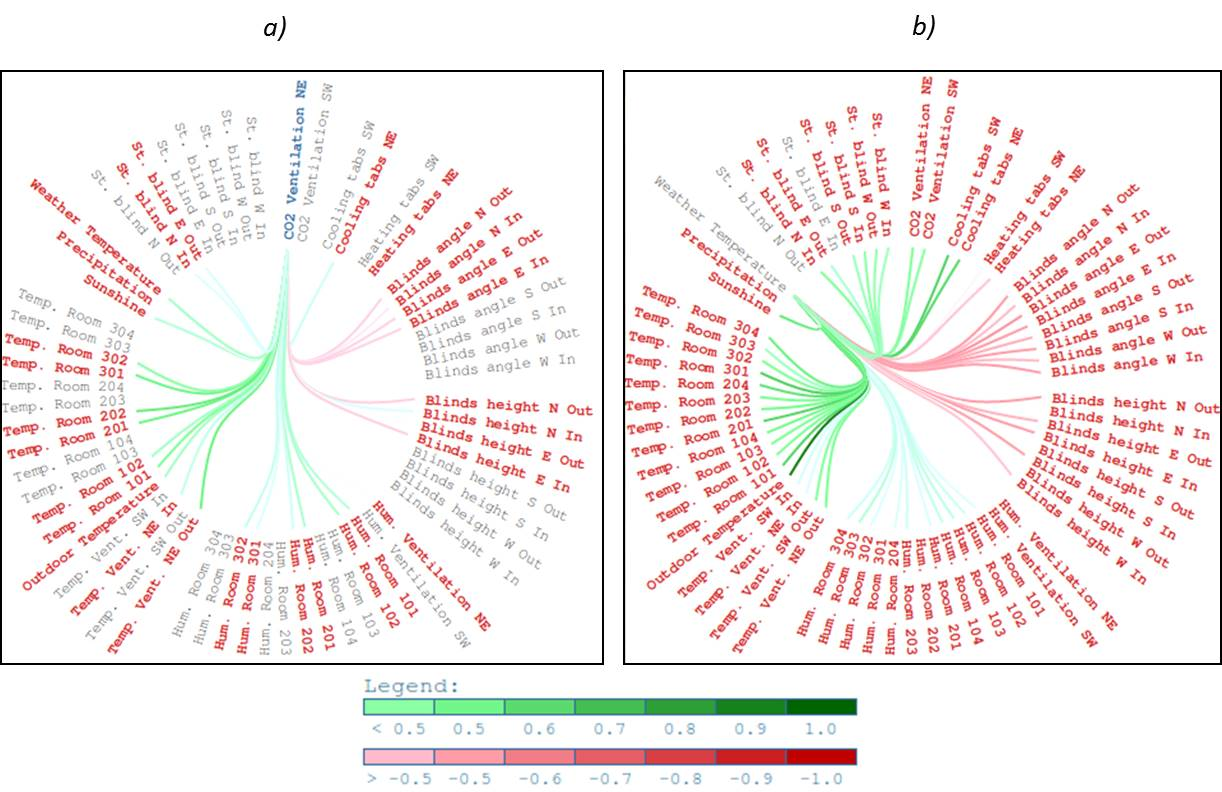
\includegraphics[scale=0.65]{Figures/flor_correlation.jpg}
  \caption{Average value of the Pearson correlation coefficient for variables of the building dataset. \textit{a)} Variables correlated with the measures of $CO_2$ levels of the North-East ventilation system. \textit{b)} Variables correlated with the weather temperature measures.}
  \label{fig:edge}
\end{figure}


\begin{figure}[h!]
  \vspace{0.5em} %better style
  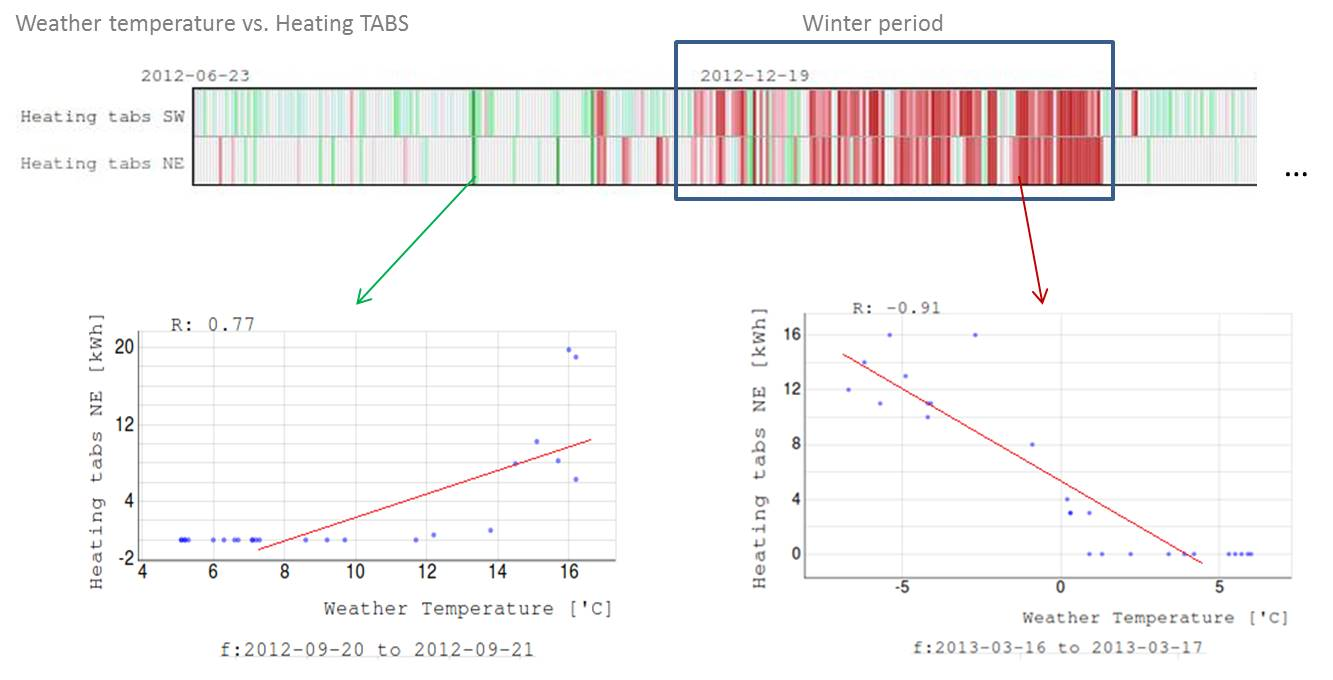
\includegraphics[scale=0.65]{Figures/heatmap.jpg}
  \caption{Average value of the Pearson correlation coefficient for variables of the building dataset. \textit{a)} Variables correlated with the measures of $CO_2$ levels of the North-East ventilation system. \textit{b)} Variables correlated with the weather temperature measures.}
  \label{fig:heatmap}
\end{figure}

The average value of the Pearson correlation coefficient is calculated by equation \ref{aver} where $X_i$ and $Y_i$ are a daily time series, and $L$ is total number of daily time series. Figure \ref{fig:edge} shows in red and green colors, the average values of $r$ during the entire timeline. The green color implies a positive correlation while the red implies a negative correlation between variables. The reason for a pair of variables having a $\overline{r}$ value close to zero, is because there is either no correlation between them or because the correlation changes frequently depending on the season and/or the day of the week (i.e. going from positive to negative and vice versa). This is the case for instance of the correlation between weather temperature (°C) and heating TABS energy consumption (kWh). Figure \ref{fig:heatmap} refers to the aforementioned case. It  is clear to see how the correlation between these two variables changes during the winter period. Furthermore, the fact that the
heating TABS of the South-West part of the building has more slightly positive correlation than the North-East part (when not in the winter period), is remarkable. This is the reason why the $\overline{r}$ value for the south-west TABS is close to zero (see \ref{fig:edge} {\color{red} .\textit{b)}}).  

The \textit{GaHMM - interactional} model uses the information from the matrix $R$. Each observed samples $O_i$ is defined by a vector called $R_{vector}$. This vector contains the $r$ value for variables of interest. 

\begin{equation}
O_i = R_{vector} (X_i) = [r(X_i,X_1), r(X_i, X_2), ..., r(X_i, X_n)]
\label{r_vector}
\end{equation}

For our proposed model, $X_i$ refers to the $CO_2$ levels of the North-East or South-West ventilation systems. The variables $X_1, ..., X_n$ correspond to different zones of the building (i.e. North-East or South-West). In this way, two $R_{vector}$ are defined for each zone in a daily fashion. Since the observed sample $O_i$ is defined, the training process can be performed according to section \ref{sec:training_process}. The evaluation and results of this model are exposed and discussed on sections \ref{sec:interactional_evaluation}, \ref{sec:interactional_results}.  


\section{Hierarchical Agglomerative Clustering}
\label{sec:hierar_agg}


In this section, we adapt the concepts that were explained in section \ref{hierarchical}, therefore in our context, an object is called a cluster profile. Since clustering is the grouping of similar objects, one can use different measures to determine whether two objects are similar or dissimilar. There are two main type of measures used to estimate similarity: distance measures and similarity measures \cite{maimon2007soft}. Normally, distance measures are used for determining the similarity between two objects in the HAC approach. Here a brief list of some of them: \textit{Euclidean distance, squared Euclidean distance, city-block (Manhattan) distance, Chebychev distance, power distance, Mahalanobis distance}. We do not go in details about each dissimilarity/similarity distance, the reader can find details in \cite{maimon2007soft,saraccli2013comparison,mullner2011modern}. However we consider important to add the definition of the euclidean distance (equation \ref{equa1}), for exemplification purposes: 

\begin{equation}
\label{equa1}
 \displaystyle d(p,q)={\sqrt {(p_{1}-q_{1})^{2}+(p_{2}-q_{2})^{2}+\cdots +(p_{i}-q_{i})^{2}+\cdots +(p_{n}-q_{n})^{2}}} 
\end{equation} 

$d(p,q)$ is the euclidean distance of two daily profiles $p$ and $q$, where $p_i$ corresponds to a measure value that belongs to the daily profile $p$. The Hierarchical agglomerative clustering creates a distance matrix $D$ using a distance measure. For example, table \ref{fig:matrix_1} is the distance matrix of 5 hypothetical daily profiles, where profiles 3 and 5 are the closest ones. This implies the first hierarchical cluster (i.e. $id= 35$). 

\begin{figure}[h!]
  \vspace{0.5em} %better style
  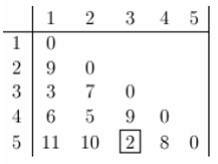
\includegraphics[scale=0.65]{Figures/distance_matrix_1.jpg}
  \caption{Distance matrix $D$ of 5 hypothetical daily profiles, using the euclidean distance. First interaction.}
  \label{fig:matrix_1}
\end{figure}

Now the distance between any cluster profile against the hierarchical cluster $id=35$ should be defined. This new similarity distance between hierarchical nodes is what is called as linkage method. There are different methods for linkage: \textit{Single link, Complete link, Group average, Ward’s method, etc.}. The reader is invited to refer more information about linkage methods in \cite{maimon2007soft,saraccli2013comparison,mullner2011modern}. We include in equation \ref{equa2} the group average linkage method, for illustration purposes:

\begin{equation}
\label{equa2}
    d ( A , B ) = \dfrac{1}{|A| \cdot |B|} \sum_{p \in A} \sum_{q \in B} d(p,q)
\end{equation} 

$d(A ,B)$ implies the distance that exists between hierarchical clusters $A$ and $B$ using the average linkage method. A hierarchical cluster collapse similar objects where dissimilarity distance is the smallest. Table \ref{fig:matrix_2} shows the case when the profile cluster $3$ and $5$ are collapsed in one hierarchical cluster $35$. The distances within the distance matrix $D$ are calculated by using equation \ref{equa2}.  

\begin{figure}[h!]
  \vspace{0.5em} %better style
  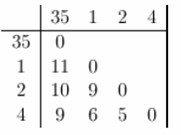
\includegraphics[scale=0.65]{Figures/distance_matrix_2.jpg}
  \caption{Distance matrix $D$ of 5 hypothetical daily profiles, using the euclidean distance. Second interaction.}
  \label{fig:matrix_2}
\end{figure}

In a new interaction, the new hierarchical cluster is $ID=24$ since the distance between profile $2$ and $4$ is the shortest one. New interactions are performed until the total reduction of the distance matrix $D$. The result of the hierarchical clustering can be displayed in a tree-like structure, called a dendrogram (see figure \ref{fig:dendogram_total}), with one cluster at the top containing all the objects, and each branch groups similar objects. 

\begin{figure}[h!]
  \vspace{0.5em} %better style
  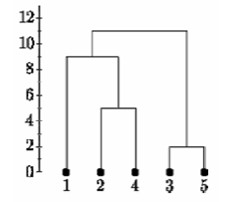
\includegraphics[scale=0.65]{Figures/dendogram_result.jpg}
  \caption{Resulting dendrogram from the distance matrix $D$.}
  \label{fig:dendogram_total}
\end{figure}


This is the process to perform a hierarchical agglomerative clustering with cluster profiles. We indicate in a practical way, how this clustering is performed in section \ref{sec:discord_finding}. In addition, a measure (i.e. \textit{Cophenetic correlation coefficient}) for knowing how faithfully a dendrogram preserves the pairwise distances between the original unmodeled data points is used. This measure allows to know which distance metric and linkage method is the most appropriated for the data \cite{saraccli2013comparison}. 

\section{Evaluation}
\label{sec:eval_all}

\subsection{Evaluation of the \textit{GaHMM - profile} model}
\label{sec:profile_evaluation}

Our approach trains a \textit{GaHMM-profile model} for each variable of the data set. This training process is done according to \ref{sec:training_process} \footnote{Script: \textit{4.hmm\_learning\_per\_variable\_k-fold.py}}. The best model is elected by using the log probability of $ p(\mathbb{O}|\lambda)$ and the results are presented as the average of $p(\mathbb{O}|\mathbb{S})$. A box plot is proposed to see the quality of the cluster profiles. Figure \ref{fig:box_plot} shows \textbf{a)} a profile cluster of a poor trained \textit{GaHMM - profile} (i.e. $\overline{p}(\mathbb{O}|\mathbb{S}) = 0.885 $, $n_{component}=9$ ) of the $CO_2$ measures of the North-East ventilation system,  one can see the amount of outliers (i.e. fliers) outside of the whiskers, in contrast with \textbf{b)} a profile cluster of the best trained \textit{GaHMM - profile} (i.e. $\overline{p}(\mathbb{O}|\mathbb{S}) = 0.993 $, $n_{component}=33$) where there are only 4 outliers.   

\begin{figure}[h!]
  \vspace{0.5em} %better style
  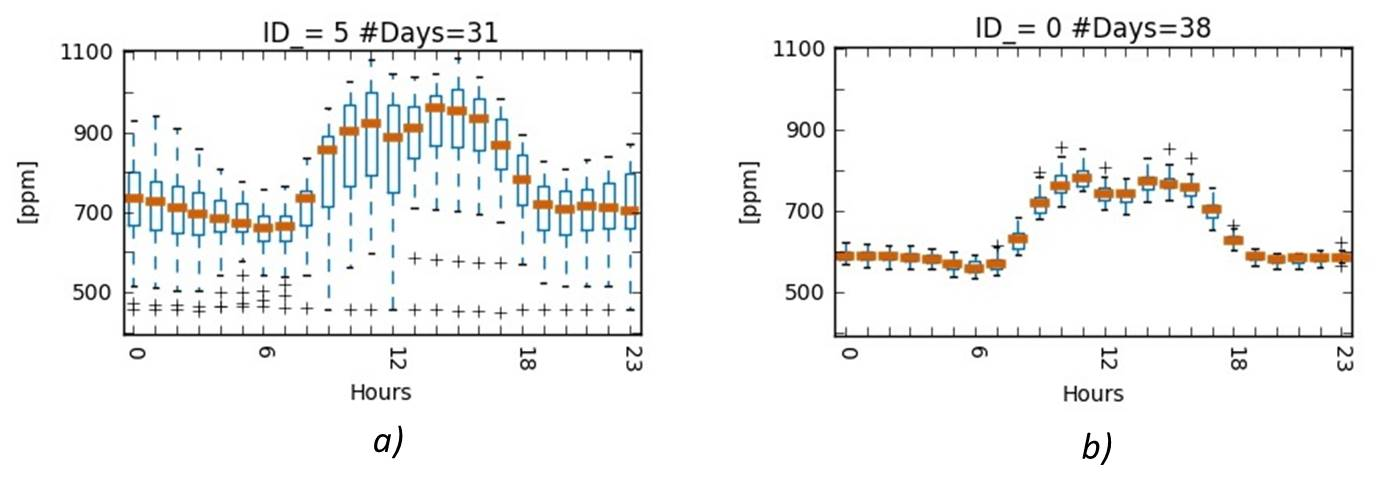
\includegraphics[scale=0.65]{Figures/box_plot.jpg}
  \caption{ $CO_2$ cluster profile of 
  a)  \textit{GaHMM - profile} with $\overline{p}(\mathbb{O}|\mathbb{S}) = 0.885, n_{component}=9 $ b) \textit{GaHMM - profile} with $\overline{p}(\mathbb{O}|\mathbb{S}) = 0.993, n_{component}=33$.}
  \label{fig:box_plot}
\end{figure} 


It follows then that, cluster profiles which belong to the best \textit{GaHMM - profile} models have tiny standard deviations for each hour of the day and there are no outliers (the number of outliers is less than 10\% of the whole samples). In this way, one obtains a good representation of the existing daily profiles. This is how each \textit{GaHMM - profile} model is evaluated. Table \ref{tab:profile_model_eval} shows the evaluation of the models that are used in a
case study (section \ref{section:CO2_analysis}). Additionally, one can see the quality of clusters in annex \ref{cluster_profiles} and the digital folder annex: iPythonBooks/Diversity of profiles.


% Table generated by Excel2LaTeX from sheet 'Hoja2'
\begin{table}[htbp]
  \centering
  \scriptsize
  \caption{Example of evaluation of \textit{GaHMM - profile} models for different variables}
    \begin{tabular}{|l|r|r|r|r|r|}
    \hline
    Variable & \multicolumn{1}{l|}{TABS Cooling NE} & \multicolumn{1}{l|}{TABS Heating NE} & \multicolumn{1}{l|}{Exhaust Air Temperature} & \multicolumn{1}{l|}{Intake air temperature} & \multicolumn{1}{l|}{$CO_2$ NE} \bigstrut\\
    \hline
    $\overline{p}(\mathbb{O}|\mathbb{S})$ & 0.9997 & 0.9982 & 0.9963 & 0.9976 & 0.9932 \bigstrut\\
    \hline
    $n_{components}$ & 33   & 32   & 31   & 33   & 33 \bigstrut\\
    \hline
    \end{tabular}%
  \label{tab:profile_model_eval}%
\end{table}%


\subsection{Evaluation of the \textit{GaHMM - seasonal} model}
\label{sec:seasonal_evaluation}


A \textit{GaHMM - seasonal} model is trained according to section \ref{sec:training_process} \footnote{script \textit{4.hmm\_learning\_k-fold.py}}  and \ref{sec:seasonal_model}. To evaluate a \textit{GaHMM - seasonal} model, we propose the use of log probability of $ p(\mathbb{O}|\lambda)$, average of $p(\mathbb{O}|\mathbb{S})$ and a visualization of the $S_{vector}$ in 3D space by using PCA. Table \ref{tab:result_training_seasonal} shows the evaluation of the best trained models for different number of features $ f $ and different number of hidden states $n$ according to sections \ref{sec:training_process} and \ref{sec:seasonal_model}. The selected variables for this table are the outdoor temperature of the building and the weather temperature. One can observe that the average of $p(\mathbb{O}|\mathbb{S})$ improves as we add new features but this diminishes after $f = 6$. The tendency is that the more features and variables we use to train the model, the more hidden states we need to describe the clusters. The observed sample $O_i$ becomes more scattered and therefore more clusters are needed, however even if we increase the number of hidden states, we do not get the same results that were achieved by the model with $f = 6$ and
$n = 2; 3; 4$.

Since the best results are achieved with $n=2,3,4$, we can choose to group the seasonal patterns in 2 or 3 or 4 clusters. We decide to group the patterns in four latent groups. They were named as \textit{summer, winter, coldest transition and hottest transition} due to the distribution of each cluster, this can be observed in figure \ref{fig:monthly}. Notice that names spring and autumn were not included in the list because when one sees the monthly distribution of the clusters, one can observe that the seasonal period of spring and autumn share some patterns in common. This last fact is explained further on section \ref{sec:seasonal_results}. 



%-------------------------------------------
%------------------------------------------------------------

% Table generated by Excel2LaTeX from sheet 'Feature Selection'
\begin{table}[htbp]
  \centering
  \scriptsize
  \caption{Average of $p(\mathbb{O}|\mathbb{S})$ for different \textit{GaHMM} models using $f$ features of outdoor temperature and weather temperature variables. }
      \begin{tabular}{|l|r|r|r|r|r|r|r|r|r|}
    \hline
         & \multicolumn{1}{l|}{f = 3} & \multicolumn{1}{l|}{f = 4} & \multicolumn{1}{l|}{f = 5} & \multicolumn{1}{l|}{f = 6} & \multicolumn{1}{l|}{f = 7} & \multicolumn{1}{l|}{f = 9} & \multicolumn{1}{l|}{f = 10} & \multicolumn{1}{l|}{…} & \multicolumn{1}{l|}{f = 18} \bigstrut\\
    \hline
    n = 2 & \cellcolor[rgb]{ .773,  .851,  .945} \textbf{0.99109447} & 0.99153911 & 0.99178444 & \cellcolor[rgb]{ 1,  .753,  0} \textbf{0.99859934} & 0.98443497 & 0.98467069 & 0.97706896 &      & 0.9924231 \bigstrut\\
    \hline
    n = 3 & 0.98247032 & \cellcolor[rgb]{ .773,  .851,  .945} \textbf{0.99248157} & \cellcolor[rgb]{ .773,  .851,  .945} \textbf{0.99339644} & \cellcolor[rgb]{ 1,  .753,  0} \textbf{0.99963577} & 0.9746971 & 0.97469422 & 0.969422 &      & 0.9974565 \bigstrut\\
    \hline
    n = 4 & 0.97436977 & 0.98552845 & 0.98819893 & \cellcolor[rgb]{ 1,  .753,  0} \textbf{0.99889142} & \cellcolor[rgb]{ .773,  .851,  .945} \textbf{0.98574802} & \cellcolor[rgb]{ .773,  .851,  .945} \textbf{0.98505652} & 0.96177504 &      & 0.9956667 \bigstrut\\
    \hline
    n = 5 & 0.97249754 & 0.98488397 & 0.98415621 & 0.99113528 & 0.98121257 & 0.9791666 & \cellcolor[rgb]{ .773,  .851,  .945} \textbf{0.9791666} &      & \cellcolor[rgb]{ .773,  .851,  .945} \textbf{0.9992562} \bigstrut\\
    \hline
    \end{tabular}%
  \label{tab:result_training_seasonal}%
\end{table}%

\begin{figure}[h!]
  \vspace{0.5em} %better style
  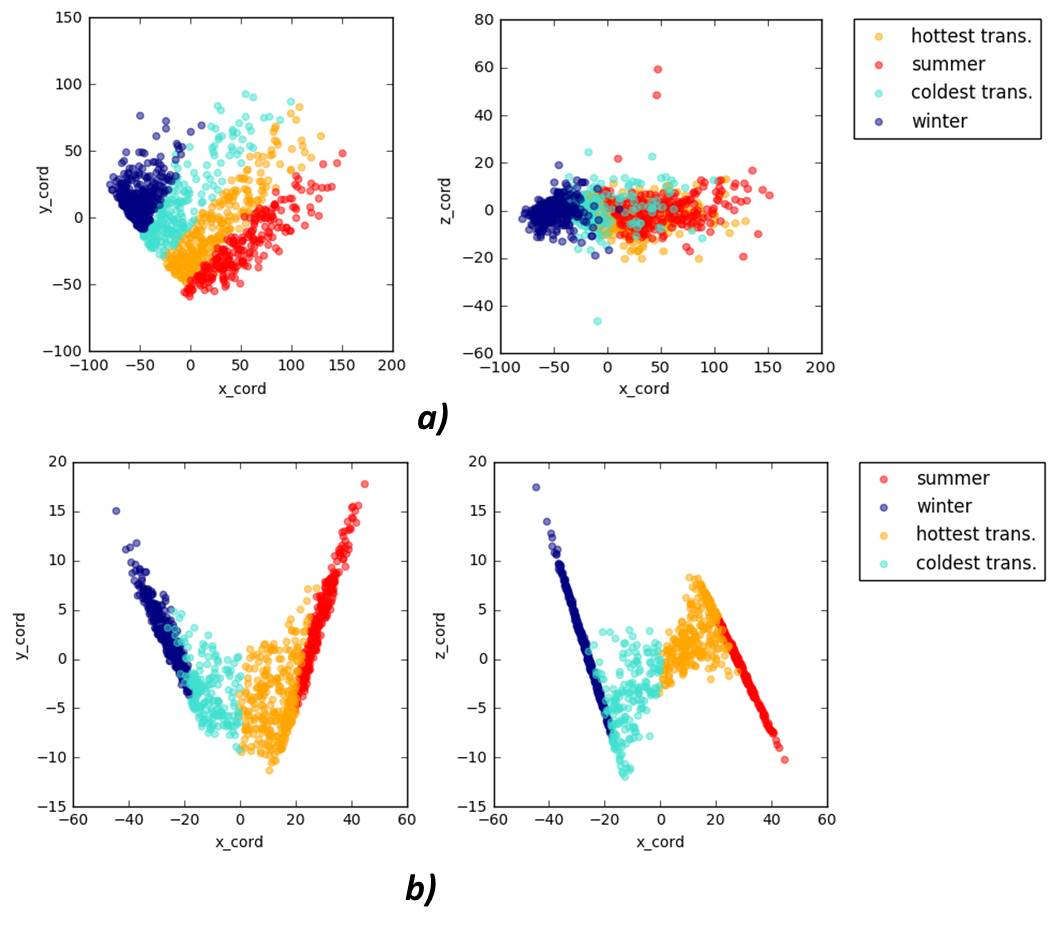
\includegraphics[scale=0.73]{Figures/PCA_visualization_C1-C4.jpg}
  \caption{Dimensional reduction using PCA for visualization: a) Visualization of $S_{vector}$ with 18 features b) Visualization of $S_{vector}$ with 6 features. Colors according to the trained \textit{GaHMM} seasonal models.}
  \label{fig:PCA_visualization}
\end{figure} 


One can observe the last fact by using the PCA procedure to transform the $S_{vector}$ to a new coordinate system, in this way, one can appreciate the quality of the clusters and the dispersion of the $S_{vector}$. Figure \ref{fig:PCA_visualization} shows the difference when \textbf{a)} we use a $S_{vector}$ of 18 features according
to annex \ref{tab:feature_list} and \textbf{b)} when we use a $S_{vector}$ of 6 features that have a good gain of information\footnote{The gain of information (i.e. entropy) was calculated and saved in 'feature\_selection' collection} according to \ref{sec:feature_selection}. Figure \ref{fig:PCA_visualization}{\color{red} .\textit{b)}} shows how the 6 features represent a good clustering quality. The results of the best GaHMM seasonal models are explained in section \ref{sec:seasonal_results}. 


\subsection{Evaluation of the \textit{GaHMM - interactional} model}
\label{sec:interactional_evaluation}

A \textit{GaHMM - interactional} model is trained according to section \ref{sec:training_process} \footnote{script \textit{4.hmm\_learning\_k-fold.py}} and \ref{sec:interactional_model}. To evaluate a \textit{GaHMM - interactional} model, we propose the use of log probability of $ p(\mathbb{O}|\lambda)$, average of $p(\mathbb{O}|\mathbb{S})$ and a visualization of the $R_{vector}$ in 3D space by using PCA. Table \ref{tab:result_interactional} shows the evaluation of the best trained models for different variables in $V_1$ and the different number of hidden states $n$ according to sections \ref{sec:training_process} and \ref{sec:interactional_model}. Each category is a group of different variables as is shown in annex (\ref{sec:metadata_t}, \textit{breakout\_group}).


% Table generated by Excel2LaTeX from sheet 'Category_selection'
\begin{table}[htbp]
  \centering
  \scriptsize
  \caption{$\overline{p}(\mathbb{O}|\mathbb{S})$ for each \textit{GaHMM interactional} model. The code of the selected categories are in annex \ref{sec:metadata_t}. These categories belongs to the North-East part of the building.}
    \begin{tabular}{|l|r|r|r|r|}
    \hline
    \textit{\textbf{Selected Categories}} & \multicolumn{1}{l|}{\textit{\textbf{n=2}}} & \multicolumn{1}{l|}{\textit{\textbf{n=3}}} & \multicolumn{1}{l|}{\textit{\textbf{n=4}}} & \multicolumn{1}{l|}{\textit{\textbf{n=5}}} \bigstrut\\
    \hline
    $[A\_6\_1, A\_6\_2, A\_6\_3]$ & \cellcolor[rgb]{ .573,  .804,  .863} 0.988713 & 0.977466 & 0.957416 & 0.960756 \bigstrut\\
    \hline
    \textcolor[rgb]{ 1,  0,  0}{$[A\_3, A\_{4\_1}, A\_{4\_2},  A\_{6\_1}, A\_{6\_2}]$} & 0.999950 & \cellcolor[rgb]{ 1,  .753,  0} 1.000000 & 0.999999 & 0.993509 \bigstrut\\
    \hline
    $[A\_{5\_1}, A\_{5\_2}, A\_{6\_1}, A\_{6\_2}, A\_{6\_3}]$ & \cellcolor[rgb]{ .573,  .804,  .863} 0.988981 & 0.976075 & 0.970061 & 0.977153 \bigstrut\\
    \hline
    $[A\_3, A\_{5\_1}, A\_{5\_2} , A\_{6\_1}, A\_{6\_2}, A\_{6\_3}]$ & 0.995121 & \cellcolor[rgb]{ .573,  .804,  .863} 0.997511 & 0.972120 & 0.979629 \bigstrut\\
    \hline
    $[A\_3, A\_{4\_1}, A\_{4\_2},  A\_{5\_1}, A\_{5\_2},  A\_{6\_3}]$ & 0.998842 & 0.997909 & \cellcolor[rgb]{ .573,  .804,  .863} 0.999975 & 0.985505 \bigstrut\\
    \hline
    $[A\_3, A\_{4\_1}, A\_{4\_2}, A\_{6\_1}, A\_{6\_2}, A\_{6\_3}]$ & \cellcolor[rgb]{ .573,  .804,  .863} 0.999599 & 0.998505 & 0.982654 & 0.984053 \bigstrut\\
    \hline
    $[A\_3, A\_{4\_1}, A\_{4\_2}, A\_{5\_1}, A\_{5\_2}, A\_{6\_1}, A\_{6\_2}]$ & \cellcolor[rgb]{ .573,  .804,  .863} 0.999978 & 0.999708 & 0.998038 & 0.985093 \bigstrut\\
    \hline
    $[A\_{4\_1}, A\_{4\_2}, A\_{5\_1},  A\_{5\_2}, A\_{6\_1}, A\_{6\_2}, A\_{6\_3}]$ & \cellcolor[rgb]{ .573,  .804,  .863} 0.992985 & 0.974719 & 0.963989 & 0.991043 \bigstrut\\
    \hline
    $[A\_3,  A\_ {4\_1}, A\_{4\_2}, A\_{5\_1}, A\_{5\_2}, A\_{6\_1}, A\_{6\_2}, A\_{6\_3}]$ & \cellcolor[rgb]{ .573,  .804,  .863} 0.993445 & 0.984509 & 0.974876 & 0.965273 \bigstrut\\
    \hline
    $[A\_1, A\_2, A\_3, A\_{4\_1}, A\_{4\_2}, A\_{5\_1}, A\_{5\_2}, A\_{6\_1}, A\_{6\_2}, A\_{6\_3}]$ & \cellcolor[rgb]{ .573,  .804,  .863} 0.999715 & 0.998432 & 0.997369 & 0.987582 \bigstrut\\
    \hline
    \end{tabular}%
  \label{tab:result_interactional}%
\end{table}%


\begin{table}[]
\centering
\scriptsize
\caption{Variables according to the category code:  \textit{[A\_3, A\_{4\_1}, A\_{4\_2},  A\_{6\_1}, A\_{6\_2}]}. The complete category code is in annex \ref{sec:metadata_t}.}
\label{code_cat}
\begin{tabular}{|l|l|}
\hline
Code    & Variables                                                                          \\ \hline
A\_3    & {[}Blinds angle N Out, Blinds angle N In, Blinds angle E Out, Blinds angle E In{]} \\ \hline
A\_4\_1 & {[}Blinds height N Out, Blinds height E In{]}                                      \\ \hline
A\_4\_2 & {[}Blinds height N In, Blinds height E Out{]}                                      \\ \hline
A\_6\_1 & {[}Temp. Vent. NE Out{]}                                                           \\ \hline
A\_6\_2 & {[}Temp. Vent. NE In{]}                                                            \\ \hline
\end{tabular}
\end{table}

The selected categories $[A\_3, A\_{4\_1}, A\_{4\_2},  A\_{6\_1}, A\_{6\_2}]$ (table \ref{code_cat}) is a group of variables that have a relevant linear correlation with the $CO_2$ levels of the North-East part of the building according to the evaluation in the table \ref{tab:result_interactional}. This fact is visible when one applies dimensionality reduction using PCA to project the $R_{vector}$ in a 3D space. Figure \ref{fig:PCA_categories} shows the PCA transformation where one appreciates the difference when \textbf{a)} $R_{vector}$ is defined by categories \textit{[A\_1, A\_2, A\_3, A\_4\_1, A\_4\_2, A\_5\_1, A\_5\_2, A\_6\_1, A\_6\_2]}, and \textbf{b)} $R_{vector}$ is defined by categories \textit{[A\_3, A\_{4\_1}, A\_{4\_2},  A\_{6\_1}, A\_{6\_2}]}. It is remarkable to see a good clustering quality in the case b) where all the three cluster are clearly defined. Clusters: [\textit{Regimen NC, Regimen WC, Regimen PC}] refers to Regimen of Negative Correlation, Weak Correlation and Positive Correlation. These clusters and the corresponding results are described in section \ref{sec:interactional_results}. As additional information, we observe the same behavior for the South-West part of the building (i.e. $V_2$ and categories $B\_*$). 

\begin{figure}[h!]
  \vspace{0.5em} %better style
  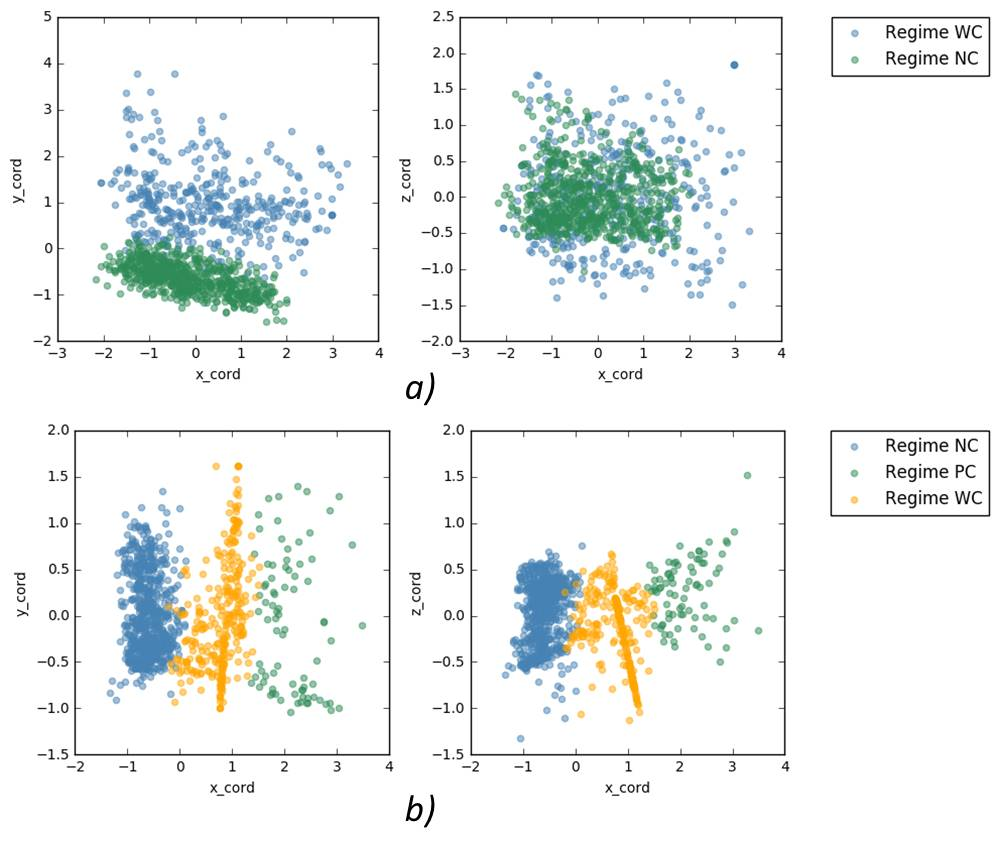
\includegraphics[scale=0.73]{Figures/Interactional_model_cluster.jpg}
  \caption{Dimensional reduction using PCA for visualization: a) Visualization of $R_{vector}$ using categories \textit{[A\_1, A\_2, A\_3, A\_4\_1, A\_4\_2, A\_5\_1, A\_5\_2, A\_6\_1, A\_6\_2]} b) Visualization of $R_{vector}$ using categories \textit{[A\_3, A\_{4\_1}, A\_{4\_2},  A\_{6\_1}, A\_{6\_2}]}. Colors according to the trained \textit{GaHMM} interactional models.}
  \label{fig:PCA_categories}
\end{figure}










